\documentclass[11pt,a4paper]{article}

\usepackage[utf8]{inputenc}
\usepackage[T1]{fontenc}
\usepackage{lmodern}
\usepackage[margin=2.3cm]{geometry}
\usepackage{amsmath,amssymb,amsthm}
\usepackage[round,authoryear]{natbib}
\usepackage{graphicx}
\usepackage{hyperref}
\usepackage{cleveref}
\usepackage{booktabs}
\usepackage{enumitem}
\usepackage{tikz}

\hypersetup{colorlinks=true,linkcolor=blue!60!black,
  citecolor=green!50!black,urlcolor=blue!70!black}

\newcommand{\ee}{\mathrm{e}}
\newcommand{\dd}{\mathrm{d}}
\newcommand{\ii}{\mathrm{i}}
\newcommand{\psit}{\tilde\psi}
\newcommand{\phit}{\tilde\phi}

\theoremstyle{plain}
\newtheorem{theorem}{Theorem}
\newtheorem{proposition}[theorem]{Proposition}
\newtheorem{conjecture}[theorem]{Conjecture}
\newtheorem{remark}[theorem]{Remark}
\newtheorem{lemma}[theorem]{Lemma}
\newtheorem{corollary}[theorem]{Corollary}

\title{Factoring the Counting Problem Out of Coupled\\
  Particle-Field Renormalisation}
\author{S. Amarteifio\\
  \small\textit{Percolation Labs}}
\date{April 2026}

\begin{document}
\maketitle

\begin{abstract}
The Doi--Peliti generating function of a reaction network, written
in the form standardly produced by the algebraic field-theoretic
formalism, is already a Lagrange equation in the sense of
Flajolet--Sedgewick analytic combinatorics.  This recognition---stated
as a theorem in the companion note~\citep{CFACtheorem}---imports
four consequences wholesale: (C1) all-orders coefficient asymptotics
via the transfer theorem, (C2) classification of mean-field
universality by the Puiseux exponent $p/q$, (C3) non-perturbative
nucleation rates as a branch-gap contour integral, and (C4) UV
divergence structure by power counting on a finite 1PI enumeration.
We call the resulting framework Coupled Field Analytic
Combinatorics (CFAC).  This paper elaborates (C1)--(C4) at
coupled-field scope on a Doi--Peliti/Martin--Siggia--Rose
Keller--Segel system and establishes three concrete results:
\textbf{Result 1}~one-loop perturbative exactness of the minimal
coupling sector, established by exhaustive 1PI graph enumeration
at $L \leq 3$---a coupled-scope sharpening of (C4);
\textbf{Result 2}~the branch-gap nucleation formula
(C3) verified to six significant figures on seven parameter sets;
\textbf{Result 3}~three-loop two-colour Kirchhoff factorisation for
every physically relevant edge colouring.  Two supporting results
extend the algebraic reach: the one-loop bridge integral has a
\emph{closed tropical form}---Arkani-Hamed--Hillman--Salvatori
leading-facet-plus-Hessian---which is exact, not asymptotic, at one
loop, and a spectral-dimension substitution $d \to d_s$ makes (C1)
and (C2) available on fractal substrates (verified on the Sierpinski
gasket to $<2\%$).  Illustrative applications to amyloid fibril
nucleation and ice crystal formation yield order-of-magnitude
estimates from published rate constants in regimes where direct
simulation cost scales as $\exp(VS)$.  Section~\ref{sec:limitations}
delimits scope: Result~2 verbatim holds only in the well-mixed
limit; a 3-site lattice test pinpoints where the real-algebraic
formulation breaks down.
\end{abstract}

% ══════════════════════════════════════════════════════════════════
\section{The counting problem is the bottleneck}
% ══════════════════════════════════════════════════════════════════

Rare nucleation events in fluctuating environments---ice crystals
in supersaturated air, amyloid fibrils at physiological monomer
concentration, bacterial colonies on surfaces---involve discrete,
countable entities in a continuous, fluctuating medium.  Two
field-theoretic traditions handle one half each.  Doi--Peliti
(DP) field theory~\cite{Doi1976,Peliti1985} derives a path
integral from a master equation; Martin--Siggia--Rose
(MSR)~\cite{MSR1973,Janssen1976,DeDominicis1976} derives one from
a stochastic PDE.  The coupled DP--MSR theory has recently been
reviewed by Pruessner and Garcia-Millan~\cite{PruessnerGarciaMillan2025}
and Bothe \textit{et al.}~\cite{Bothe2023}, who demonstrated that
coarse-grained density descriptions miss the particle structure
and produce \emph{spurious} entropy production; keeping the DP
sector is essential.

A direct renormalisation-group programme for such coupled actions
proceeds in five monolithic steps: (1) write the action; (2)
enumerate Feynman diagrams; (3) evaluate loop integrals; (4)
extract beta functions; (5) locate the instanton by complex-field
saddle point.  Steps (2)--(4) dominate the effort; step (5) is
non-perturbative and usually approached separately.  Changing
the system (different reactions, different coupling) means
redoing everything.

The point of this paper is that steps (2) and (5)---the
\emph{counting} of diagrams and the analogue for the
instanton---can be factored out.  Once factored, they reveal
structure that is hard to see in the monolithic calculation.  We
call this factorisation \textbf{Coupled Field Analytic
Combinatorics (CFAC)}.  The CFAC decomposition is
\begin{equation}\label{eq:decomposition}
  \text{Observable}
  = \underbrace{\text{Counting}}_{\text{CFAC layer}}
  \times \underbrace{\text{Bridge}}_{\text{integral table}}
  \times \underbrace{\text{Ward correction}}_{\text{symmetry}}.
\end{equation}
The CFAC layer enumerates 1PI graphs (finite), does power counting
(mechanical), builds the Dyson--Schwinger equation (DSE) and
extracts its singularity structure (algebraic).  The bridge is a
small pre-computed table of one-loop integrals indexed by topology
and $(n_\partial, m_\psi/m_\phi)$, where $n_\partial$ is the
number of gradient insertions.  The Ward layer is a finite set of
symmetry checks.

The central recognition of this paper is that the Doi--Peliti
generating function, as standardly constructed from a reaction
network, \emph{is already} a Lagrange equation of analytic
combinatorics---once one knows to look for it.  We state this as
Theorem~\ref{thm:recognition} (\S\ref{sec:recognition}) after
introducing the two technical ingredients, because the payoff is
a body of imported mathematics: the transfer theorem for
all-orders asymptotics, Puiseux classification of mean-field
universality, and a new \emph{branch-gap} contour integral for
non-perturbative nucleation rates.  The three demonstrations at
coupled-field scope---Proposition~\ref{prop:oneloop-exact}
(one-loop perturbative exactness), Theorem~\ref{thm:gap} (the
branch-gap formula), and Conjecture~\ref{conj:twocolour} (three-loop
two-colour Kirchhoff factorisation)---are all consequences of
applying Theorem~\ref{thm:recognition} to a coupled DP--MSR
system.  The acronym CFAC (Coupled Field Analytic Combinatorics)
reflects the ingredients: an algebraic formalism for
reaction-diffusion theories~\citep{Amarteifio2019Thesis} and the
analytic combinatorics of \citet{FlajoletSedgewick};
\S\ref{sec:comparison} compares CFAC with the direct-RG approach
of \citet{PruessnerGarciaMillan2025}.

% ══════════════════════════════════════════════════════════════════
\section{Background: two imported tools}
\label{sec:background}
% ══════════════════════════════════════════════════════════════════

The approach of this paper combines two bodies of work that are
largely foreign to the stochastic-field-theory mainstream and
rarely appear in the Doi--Peliti/MSR
literature~\cite{PruessnerGarciaMillan2025,Bothe2023,Tauber}.  We
introduce each separately and then describe the combination.

\subsection{Algebraic reaction-diffusion field theory}
\label{sec:algebraic}

The first ingredient is an algebraic formalism for stochastic
reaction-diffusion systems developed
in~\cite{Amarteifio2019Thesis}, building on Doi--Peliti
\cite{Doi1976,Peliti1985} and
Heisenberg--Weyl~\cite{Tauber} machinery.  The goal is to move
from \emph{deriving} field theories case-by-case (the standard
approach) to \emph{generating} them algorithmically from a
chemical reaction network.

\paragraph{Reaction network as input.}
A network is specified by its stoichiometry matrix: for each
reaction $r$, integers $k_{ri}, l_{ri}$ giving the input and
output counts of species $A_i$, together with a rate $k_r$.

\paragraph{The Doi shift and the Liouvillian.}
Each reaction $\sum_i k_{ri} A_i \to \sum_i l_{ri} A_i$ produces
the Heisenberg--Weyl contribution
\begin{equation}\label{eq:liouvillian}
  Q_r
  = k_r
  \Bigl[\prod_i (1+\psit_i)^{l_{ri}}
        - \prod_i (1+\psit_i)^{k_{ri}}\Bigr]
  \prod_i \psi_i^{k_{ri}},
\end{equation}
with $\psi_i, \psit_i$ creation/annihilation variables for
species $A_i$ (shifted by the Doi prescription~\cite{Tauber}).
Expanding~\eqref{eq:liouvillian} gives a \emph{vertex dictionary}:
each monomial $g_{\{m_i\},\{n_i\}}\prod_i
\psit_i^{m_i}\psi_i^{n_i}$ is a vertex with coupling $g$ that
depends algebraically on $k_r$ and combinatorial prefactors.

\paragraph{From vertices to diagrammatic rules.}
Feynman rules follow mechanically: each vertex $\psit^m\psi^n$
has $m$ outgoing and $n$ incoming legs; propagators connect
$\psi$ to $\psit$; symmetry factors come from graph
automorphisms.  Spatial structure enters through the free
propagator $G_0(k,\omega)^{-1} = -i\omega + Dk^2 + m$, whose
dimension fixes the upper critical dimension.  Gradient
insertions $n_\partial$ come from spatial derivatives in
interactions (drift, chemotaxis).

\paragraph{Kirchhoff polynomials from graphs.}
Every Feynman graph $\Gamma$ with $L$ loops, $I$ internal edges,
and $V$ vertices has a Kirchhoff (first Symanzik)
polynomial~\cite{BognerWeinzierl}
\begin{equation}\label{eq:kirchhoff}
  \mathcal{K}_\Gamma(\{u_e\})
  = \sum_{T \in \mathrm{ST}(\Gamma)} \prod_{e \notin T} u_e,
\end{equation}
the sum over spanning trees $T$ of products of Schwinger
parameters on edges \emph{not} in $T$.  By the matrix-tree
theorem, $\mathcal{K}_\Gamma$ equals the determinant of any
principal minor of the weighted graph Laplacian---an entirely
algebraic construction.

\paragraph{What the algebraic formalism delivers.}
Given a reaction network, this formalism produces: the vertex
dictionary; the 1PI Feynman graphs at any loop order; the
symmetry factor and Kirchhoff polynomial of each; the upper
critical dimension $d_c$; and the superficial degree of
divergence
\begin{equation}\label{eq:omega}
  \omega(\Gamma, d) = dL - 2I + n_\partial^{\mathrm{tot}}
\end{equation}
for every graph.  \emph{No loop integrals are evaluated.}

\subsection{Analytic combinatorics (Flajolet--Sedgewick)}
\label{sec:ac}

The second ingredient is analytic combinatorics (AC), a framework
developed by \citet{FlajoletSedgewick} for extracting asymptotic
behaviour of combinatorial counts from the singularity structure
of their generating functions.  AC is standard in theoretical
computer science and enumerative combinatorics (counts of trees,
graphs, paths, partitions) but is not widely used in statistical
physics, where the same asymptotic information is usually obtained
from saddle points of actions, transfer matrices, or direct
summation.

\paragraph{Why this should work for physics.}
The Doi--Peliti formulation already recasts a stochastic master
equation as an operator algebra on a Fock space, with the
Hamiltonian generating time evolution
\citep{Doi1976,Peliti1985,Tauber}.  In that language, observables
are expectation values of monomials in $\psit, \psi$; Feynman
diagrams compute them order by order; universality classes are
read off from the relevant vertices near $d_c$.  Analytic
combinatorics sits one level up: the \emph{generating function}
that resums the Feynman series is a well-defined algebraic
object---the solution of~\eqref{eq:DSE}---whose singularities
encode the universality class directly.  Three consequences
make this useful for physics.

\emph{(i) Universality classes become polynomial invariants.}
The Puiseux exponent $p/q$ at the DSE branch point classifies the
mean-field behaviour: $p/q = 1/2$ is directed percolation and
mean-field annihilation; $p/q = 1/3$ is the compact directed
percolation / triple-root regime; higher-order branch mergers
give further multi-critical points
\citep{FlajoletSedgewick,Amarteifio2019Thesis,AmarteifioBRW}.
Classification is algebraic, not dynamical.

\emph{(ii) The singularity is a handle on rare events.}
Because the transfer theorem~\eqref{eq:transfer} extracts both
rate and prefactor from the same local data, it is naturally
suited to questions about the asymptotic tails of the
perturbation series---precisely the regime where rare-event and
non-perturbative structure appear.  Theorem~\ref{thm:gap} below
makes this concrete: the nucleation barrier is a contour integral
around the DSE branch point, in the same plane where the transfer
theorem operates.

\emph{(iii) Graph-intrinsic substitution, no path integral needed.}
Reaction-diffusion on irregular substrates is notoriously awkward
in the direct field-theoretic approach: one must either redo the
RG with a non-standard propagator or appeal to scaling arguments.
In AC the spectral dimension $d_s$ enters through a single
substitution in the engineering dimensions; no propagator is
recomputed.  This is the same trick that turns Weyl's law into a
unified treatment of exponents on $\mathbb{Z}^d$, Sierpinski
carpets, random trees, and scale-free
networks~\citep{AmarteifioBRW}.

Identifying the AC constructions with stochastic-field-theoretic
quantities is the bridge we exploit.

\paragraph{Dyson--Schwinger equation as Lagrange equation.}
For a scalar field theory with vertex function
$\phi(G) = \sum_k g_k G^k$, the full propagator $G(z)$ with
source-strength $z$ satisfies the functional
equation~\cite{BognerWeinzierl}
\begin{equation}\label{eq:DSE}
  G(z) = z \cdot \phi\bigl(G(z)\bigr),
\end{equation}
a closed implicit definition of $G$ as an algebraic function of
$z$.  In AC language~\cite{FlajoletSedgewick}, \eqref{eq:DSE} is
a \emph{Lagrange equation}; the Lagrange inversion formula gives
its Taylor coefficients in closed form.

\paragraph{Branch point and Puiseux exponent.}
The implicit function theorem applied to~\eqref{eq:DSE} fails at
$(G_*, z_*)$ satisfying $1 - z_*\phi'(G_*) = 0$ and $G_* =
z_*\phi(G_*)$.  This is the \emph{branch point}.  The Newton
polygon of~\eqref{eq:DSE} near $(G_*, z_*)$ determines the local
Puiseux expansion
\begin{equation}
  G(z) - G_* \sim C\,(z_* - z)^{p/q},\qquad z \to z_*,
\end{equation}
with rational exponent $p/q$.  For a generic quadratic branch,
$p/q = 1/2$; for a triple-root merger, $p/q = 1/3$.

\paragraph{Transfer theorem.}
The central \emph{transfer theorem}~\cite{FlajoletSedgewick}
converts local singularity behaviour into asymptotic coefficient
growth:
\begin{equation}\label{eq:transfer}
  [z^n]\,G(z) \sim \frac{C}{\Gamma(-p/q)}\,n^{-p/q - 1}\,z_*^{-n},
  \qquad n \to \infty.
\end{equation}
Both the exponential rate $z_*^{-n}$ \emph{and} the algebraic
prefactor are extracted from polynomial data alone.  In the
field-theoretic interpretation, $[z^n]G(z)$ is the $n$-th
perturbative coefficient of the propagator; the transfer theorem
is the rigorous all-orders statement of the perturbation
series' singularity structure.

\paragraph{Spectral dimension.}
AC combines naturally with the spectral
dimension~\cite{AlexanderOrbach,Havlin,Hattori} of an irregular
substrate.  On a graph with spectral dimension $d_s$, the return
probability scales as $P(t) \sim t^{-d_s/2}$, and
reaction-diffusion exponents follow from $d \to d_s$ in the
engineering-dimension analysis---delivering exponents on fractals
and cellular compartments without reworking the field theory.

\subsection{Combining the two: CFAC}
\label{sec:combination}

The two ingredients are complementary.  Together they define what
we call \textbf{Coupled Field Analytic Combinatorics (CFAC)}: a
pipeline that takes a coupled-species reaction network and
returns quantitative predictions from polynomial data.  The
algebraic formalism (\S\ref{sec:algebraic}) takes a chemical
reaction network as input and produces Feynman graphs, Kirchhoff
polynomials, and the DSE.  Analytic combinatorics
(\S\ref{sec:ac}) takes the DSE as input and produces asymptotic
information: branch points, Puiseux exponents, and
transfer-theorem asymptotics.  The word \emph{coupled} in CFAC
refers both to the multi-species coupling (DP-sector particles
interacting with MSR-sector fields) and to the \emph{coupling} of
the algebraic and AC layers into a single pipeline.

Combining them turns a reaction network directly into quantitative
predictions, via the decomposition
\begin{equation}\label{eq:decomposition}
  \text{Observable}
  = \underbrace{\text{Counting}}_{\substack{\text{algebraic}\\\text{formalism + AC}}}
  \times \underbrace{\text{Bridge}}_{\text{integral table}}
  \times \underbrace{\text{Ward correction}}_{\text{symmetry}}.
\end{equation}
What AC gives that the algebraic formalism alone does not is the
all-orders singularity structure of the perturbation series:
finding the branch point of the DSE is equivalent to summing the
full series asymptotically.  What the algebraic formalism gives
that AC alone does not is the DSE in the first place---and,
crucially, the coupled DSE for a multi-species system,
constructed from the stoichiometry matrix.

\paragraph{What analytical power does AC add over conventional
pen-and-paper QFT?}
The honest answer is that AC does not reduce the intellectual work
for any \emph{single} computation; it reduces the marginal work
for each new system and exposes structural connections that are
difficult to see case-by-case.  Five concrete additions:
\begin{enumerate}[leftmargin=1.8em, itemsep=-0.2em]
\item \textit{The DSE as a closed Lagrange equation.}
  Pen-and-paper writes $G = G_0 + G_0\Sigma G$ and treats $\Sigma$
  perturbatively; AC recognises $G = z\phi(G)$ as a Lagrange
  equation, from which $[z^n]G$ follows by closed-form Lagrange
  inversion rather than iterative loop summation.
\item \textit{All-orders asymptotics via the transfer theorem.}
  Pen-and-paper gives the first few coefficients in a perturbative
  series by direct calculation.  The transfer theorem~\eqref{eq:transfer}
  gives the full $[z^n]G$ asymptotic from a local calculation at
  the branch point, including the algebraic prefactor.  This is
  the regime where Borel summation, resurgence, and
  non-perturbative structure enter.
\item \textit{Polynomial-invariant classification of universality.}
  The Puiseux exponent $p/q$ at the DSE branch point is a rational
  number determined by the polynomial structure.  $p/q = 1/2$ is
  directed percolation; $p/q = 1/3$ is the compact-DP / triple-root
  class; higher-order mergers give further multi-critical
  classes.  Classification becomes algebraic geometry on the DSE
  polynomial, not a case-by-case RG analysis.
\item \textit{Exhaustive enumeration over ``by inspection''.}
  All-orders statements in pen-and-paper QFT usually require
  resummation, induction, or symmetry arguments.  The algebraic
  formalism enumerates all 1PI graphs consistent with the vertex
  dictionary; power counting on that finite list converts an
  all-orders claim into a finite combinatorial check---as in
  Proposition~\ref{prop:oneloop-exact}.
\item \textit{A common home for perturbative and non-perturbative
  physics.}
  Pen-and-paper derives perturbative exponents from loop integrals
  and instantons from action saddle points, using distinct
  machinery.  AC places both at the branch point of the same
  generating function: the transfer theorem reads off perturbative
  asymptotics, and Theorem~\ref{thm:gap} reads off the
  non-perturbative instanton rate.  The structural identification
  is new; the numerical values it produces at $d = 0$ are not.
\end{enumerate}
For a reader familiar with pen-and-paper DP-MSR calculations, the
tangible change is that repetitive machinery (diagram
enumeration, power counting, singularity analysis) becomes
mechanical, freeing analytical effort for the genuinely
system-specific steps (identifying the vertex dictionary from the
physics, evaluating the bridge integrals, and checking Ward
identities).

\subsection{Worked example: pair annihilation}
\label{sec:worked}

For single-species pair annihilation $2A \to \varnothing$ at rate
$\lambda$ (stoichiometry $k_A{=}2$, $l_A{=}0$),
the Liouvillian~\eqref{eq:liouvillian} reads
\begin{equation}
  Q = \lambda\bigl[1 - (1+\psit)^2\bigr]\,\psi^2
  = -2\lambda\,\psit\psi^2 - \lambda\,\psit^2\psi^2,
\end{equation}
after expanding $1 - (1+\psit)^2 = -2\psit - \psit^2$.  The two
resulting interaction vertices are $(m_A, n_A) = (1, 2)$ with
coupling $-2\lambda$ and $(2, 2)$ with coupling $\lambda$; we
label them $g_{12} = -2\lambda$ and $g_{22} =
\lambda$~\citep{Doi1976,Peliti1985}.  A Pruessner-familiar reader
will recognise these as the standard DP vertices for pair
annihilation.

The mapping from these vertices to the DSE kernel $\phi(G)$
is the point where the algebraic formalism meets analytic
combinatorics, and is worth spelling out.  In the DSE~\eqref{eq:DSE},
$G(z)$ is the full (dressed) particle propagator,\footnote{More
precisely, $G(z)$ is the generating function
$\sum_n n!\,\langle\psi^n\psit^n\rangle\,z^n$ of equal-time connected
correlators in the DP path integral; $z$ is the source strength.
In AC language it is the \emph{Lagrange generating function} for
rooted 1PI trees~\citep{FlajoletSedgewick,BognerWeinzierl}.}
and $z$ the bare propagator.  Summing over all 1PI insertions,
each interaction vertex $\psit^m\psi^n$ attaches to a vertex of
$G$ by contracting one $\psit$-leg (to the external line) and
$(m-1)$ $\psit$-legs and $n$ $\psi$-legs to internal dressed
propagators---giving a contribution $g_{mn}\,G^{m+n-2}$.  Summing
all vertices plus the identity:
\begin{equation}\label{eq:phi-from-vertices}
  \phi(G) = 1 + \sum_{m,n:\,m+n\geq 3} g_{mn}\,G^{m+n-2}.
\end{equation}
For pair annihilation: $\phi(G) = 1 + g_{12}G + g_{22}G^2 =
1 - 2\lambda G + \lambda G^2$.  The DSE~\eqref{eq:DSE} is
therefore $G = z\bigl[1 - 2\lambda G + \lambda G^2\bigr]$, a
quadratic in $G$.

Solving: the branch point is at $G_* = 1/\lambda$,
$z_* = 1/\lambda$; the Puiseux exponent is $1/2$.  The transfer
theorem~\eqref{eq:transfer} gives $[z^n]G(z) \sim
n^{-3/2}\lambda^n$.  Combined with Weyl's law on $\mathbb{Z}^d$
(substitution $d \to d_s$), this recovers the mean-field density
decay $\rho(t) \sim t^{-d/2}$ for $d \geq 2$ and its breakdown
for $d < 2$~\citep{Tauber}.  A fully worked example for the
Gribov/BRW process ($A \to 2A$, $2A \to A$, $A \to \varnothing$)
is given in a companion note~\citep{AmarteifioBRW}.  \emph{No
loop integral was evaluated in either case.}

\subsection{Main recognition theorem}
\label{sec:recognition}

The preceding subsections separately developed the algebraic
reaction-diffusion formalism (\S\ref{sec:algebraic}) and analytic
combinatorics (\S\ref{sec:ac}).  The central observation of this
paper is that the object they share is already the same:

\begin{theorem}[CFAC recognition]
\label{thm:recognition}
Let a reaction network have polynomial vertex structure (all
vertices arising from the Doi--Peliti expansion of a finite
stoichiometry matrix, projected if necessary to zero spatial
dimensions).  Then the Doi--Peliti dressed-propagator generating
function $G(z)$, constructed from the Liouvillian of the network
by the standard second-quantised field-theoretic route, satisfies
\begin{equation}\label{eq:recognition}
  G(z) = z\cdot\phi\bigl(G(z)\bigr),
  \qquad
  \phi(G) = 1 + \sum_{m + n \geq 3} g_{m n}\,G^{m + n - 2},
\end{equation}
with $\phi$ a polynomial determined algorithmically by the
stoichiometry.  Equation~\eqref{eq:recognition} is a Lagrange
equation in the sense of analytic combinatorics
\citep{FlajoletSedgewick}.  Consequently:
\begin{enumerate}[leftmargin=1.8em, itemsep=-0.2em]
\item \textit{All-orders coefficient asymptotics} are given by the
  transfer theorem~\eqref{eq:transfer}, with exponential rate
  $z_*^{-n}$ and algebraic prefactor set by the Puiseux exponent
  at the branch point.
\item \textit{Mean-field universality classes} are indexed by the
  Puiseux exponent $p/q$, a rational invariant of the polynomial
  $\phi$ at its branch point.
\item \textit{Non-perturbative nucleation rates} are extracted by
  the branch-gap contour
  integral~\eqref{eq:branch-gap} of the same polynomial
  (Theorem~\ref{thm:gap} below).
\item \textit{Higher-loop UV divergences} are classified by the
  superficial degree of divergence
  $\omega = dL - 2I + n_\partial^{\mathrm{tot}}$ evaluated on the
  finite enumeration of 1PI graphs consistent with the vertex
  dictionary.
\end{enumerate}
\end{theorem}

\paragraph{Why this is the whole paper.}
For a reader familiar with Doi--Peliti, steps (1)--(4) are not
usually thought of as properties of a single object.  They are
handled by separate technical routes: loop integration and RG for
perturbative exponents, action saddle-points for non-perturbative
rates, case-by-case dimensional analysis for universality classes.
Theorem~\ref{thm:recognition} says they are all consequences of
the \emph{same} polynomial~$\phi(G)$---the one that drops out of
the algebraic formalism as soon as the Liouvillian is expanded.
The physicist's DP generating function and Flajolet--Sedgewick's
Lagrange equation are the same object, and the Flajolet--Sedgewick
theorem apparatus transfers.

This is the clean content.  The rest of the paper demonstrates the
three non-trivial consequences at coupled-field scope:
Proposition~\ref{prop:oneloop-exact} is (4) applied to the
coupled Keller--Segel sector; Theorem~\ref{thm:gap} is (3) proved
via change of variables; Conjecture~\ref{conj:twocolour} is a
structural claim about how (4) behaves under bi-colouring of edges.

\paragraph{Scope.}
The theorem as stated holds when $\phi$ is polynomial in $G$
alone.  This covers pure reaction networks (DP) and the
field-integrated projections of coupled theories used in
Theorem~\ref{thm:gap}.  When gradient vertices carry
momentum-dependent couplings (as in the spatially resolved
coupled theory of~\S\ref{sec:oneloop-exact}), $\phi$ depends on
momentum and the recognition becomes a functional statement; the
transfer-theorem apparatus extends but is more involved.  All
coupled-field applications in this paper either project to $d = 0$
(nucleation, \S\ref{sec:applications}) or are single-loop
perturbative (\S\ref{sec:oneloop-exact}), so the polynomial form
of Theorem~\ref{thm:recognition} is sufficient.

% ══════════════════════════════════════════════════════════════════
\section{Test case: coupled Keller--Segel}
% ══════════════════════════════════════════════════════════════════

We take bacterial chemotaxis~\cite{KellerSegel1970} as the vehicle.
Discrete bacteria $\psi$ diffuse ($D_A$) and are biased by an
attractant field $\phi$ (diffusion $D_c$, decay $\kappa$).
Bacteria source the field at rate $\mu$; the gradient biases
their motion with strength $\chi$.  The coupling is
\begin{equation}\label{eq:KS-vertices}
  S_{\mathrm{int}}
  = -\chi\!\int\!\psit\,(\nabla\phi)\!\cdot\!(\nabla\psi)
  - \mu\!\int\!\phit\,\psit\,\psi.
\end{equation}
The chemotaxis vertex has $n_\partial = 2$; the secretion vertex
has $n_\partial = 0$.  Saddle points reproduce the classical
Keller--Segel PDE; linearising gives the mean-field instability
threshold $n_c = D_A\kappa/(\chi\mu)$.

The direct-RG calculation for a related model was carried out by
Gelimson and Golestanian~\cite{GelimsonGolestanian2015}; they
integrated out the field first, obtaining a long-range Coulomb
interaction, then applied RG to the single resulting field.  We
retain both fields explicitly.

% ══════════════════════════════════════════════════════════════════
\section{CFAC result 1: one-loop perturbative exactness}
\label{sec:oneloop-exact}
% ══════════════════════════════════════════════════════════════════

\subsection{The perturbative sector is pure bi-coloured graph theory}

At the level of diagrams, a coupled DP--MSR theory is a field
theory with two propagator types (DP and MSR, bi-coloured) and a
vertex dictionary read off from the Liouvillian.  Every
perturbative observable---exponents, beta functions, fixed
points---is determined by three algebraic data attached to each
1PI graph: the graph topology, its Kirchhoff polynomial
$\mathcal{K}_\Gamma(\{u_e\})$ with edges coloured DP or MSR, and
the Symanzik polynomial containing the propagator masses
$m_\psi$, $m_\phi$ and diffusion constants $D_A$, $D_c$.

\begin{proposition}[Perturbative coupled-field theorem]
\label{prop:perturbative}
For any coupled DP--MSR reaction network with polynomial vertex
structure, the full perturbative renormalisation-group flow is
determined by the bi-coloured Kirchhoff and Symanzik polynomials
on the enumerated 1PI graphs.  Specifically:
\begin{enumerate}[leftmargin=1.8em, itemsep=-0.2em]
\item 1PI graphs at loop order $L$ are enumerated by the algebraic
  formalism from the vertex dictionary (finite list per $L$).
\item Each graph has a two-colour Kirchhoff polynomial
  $\mathcal{K}_\Gamma(p, f)$ (matrix-tree theorem on the
  weighted Laplacian with edge colours $p = G_\psi$,
  $f = G_\phi$).
\item The superficial degree of divergence
  $\omega(\Gamma, d) = dL - 2I + n_\partial^{\mathrm{tot}}$
  classifies which graphs are UV divergent; the finite list of
  divergent graphs determines the beta functions at each loop
  order.
\item Mass ratios $(m_\psi/m_\phi)$ and diffusion ratios
  $(D_A/D_c)$ enter only through the Symanzik polynomial
  evaluated at the saddle; bi-coloured factorisation
  (Conjecture~\ref{conj:twocolour}) splits these dependencies
  into single-colour factors.
\end{enumerate}
\end{proposition}

\paragraph{Significance.}
The proposition generalises Result 1 below from the KS-specific
coupling to an arbitrary coupled DP--MSR reaction network with
polynomial vertices.  Every such system is handled by the same
algebraic pipeline; only the Kirchhoff- and Symanzik-polynomial
inputs change.  KS, a field-coupled Schl\"ogl model, coupled
catalysis networks, multi-species chemotaxis---the
\emph{perturbative} RG flow of all of these is determined by the
same construction, with no case-by-case derivation of Feynman
rules.  The one-loop exactness of the minimal KS coupling sector
(Corollary~\ref{prop:oneloop-exact} below) is a specific instance
in which the vertex content is so constrained that the divergent
graph list is finite even at all orders.

\subsection{Corollary: one-loop exactness of the minimal KS
coupling sector}

\begin{proposition}[One-loop perturbative exactness of the
coupling sector]
\label{prop:oneloop-exact}
Consider the minimal coupled theory defined by the two coupling
vertices in~\eqref{eq:KS-vertices} together with free DP and MSR
propagators and \emph{no additional interaction vertices}
(i.e.\ no DP branching/death or MSR noise vertices).  The
bacterial self-energy of this theory has a single UV divergence
at one loop,
\begin{equation}\label{eq:deltaDA}
  \delta D_A^{(1)}
  = +\frac{\chi\mu\,D_c D_A}{\pi(D_A+D_c)^3}\,\frac{1}{\varepsilon}
  + O(\varepsilon^0), \quad \varepsilon = 2 - d,
\end{equation}
and \emph{no} UV divergences at any loop order $L \geq 2$.
All vertex corrections and the attractant self-energy are UV
finite; $Z_\chi = Z_\mu = Z_\phi = 1$; the beta function of
$g = \chi\mu/[2\pi(D_A+D_c)^2]$ is
\begin{equation}\label{eq:beta}
  \beta_g
  = -\varepsilon g - \frac{4 D_A D_c}{(D_A+D_c)^2}\,g^2
\end{equation}
\emph{exactly} to all perturbative orders in this minimal sector.
\end{proposition}

\paragraph{Scope.}
The proposition is a statement about the \emph{coupling sector}
of the KS theory only.  Adding DP branching ($\psit^2\psi$, which
governs the directed-percolation universality class~\cite{Tauber})
or DP death ($\psit\psi$ mass term) introduces additional
vertices that enumerate to new divergent graphs at higher loop
orders; the all-orders $\omega_L < 0$ bound derived below no
longer holds uniformly.  Adding MSR noise ($\phit^2$) modifies
the attractant self-energy.  Result 1 therefore isolates the
perturbative behaviour of the \emph{coupling alone}, disentangled
from the well-studied DP and MSR divergences.

\paragraph{What CFAC does, and what a human/code does at each step.}
The proposition claims an \emph{all-orders} statement: that no UV
divergence exists beyond one loop.  In the direct-RG route, this
would require computing a potentially infinite sequence of
integrals; CFAC reduces it to a finite, mechanical inspection.
Concretely, the pipeline is:
\begin{enumerate}[leftmargin=1.8em, itemsep=-0.2em]
\item \textit{Input (human):} the vertex dictionary from
  \eqref{eq:KS-vertices}---two coupling vertices $\chi$ (3-leg,
  $n_\partial = 2$) and $\mu$ (3-leg, $n_\partial = 0$), plus the
  free DP and MSR sectors.
\item \textit{Counting $L$ (algebra):} for 3-leg vertices and
  $E = 2$ external legs, leg-counting $3V = 2I + E$ plus the
  Euler relation $L = I - V + 1$ give $V = 2L$, $I = 2L + 1$ at
  loop order $L$.  Two lines of algebra.
\item \textit{Graph enumeration (code):} enumerate all
  non-isomorphic 1PI graphs with these $(V, I, E)$ and compatible
  leg types.  At $L = 2$: the unique topology is $K_4 \setminus e$;
  at $L = 3$: the unique topology is the triangular prism (after
  automorphism).  Vertex-consistent edge colourings are enumerated
  directly (\texttt{paper/reproduce.py}, $\sim 10$ lines of
  \texttt{sympy}).
\item \textit{Power counting (algebra):} apply
  $\omega = 2L - 2I + n_\partial^{\mathrm{tot}}$ to each coloured
  graph.  One subtraction per diagram.
\item \textit{Verdict (by inspection):} every diagram at
  $L \geq 2$ has $\omega < 0$, so every diagram at $L \geq 2$ is
  UV convergent.
\end{enumerate}

\paragraph{What $\omega$ is doing, and why the inspection is justified.}
The superficial degree of divergence
$\omega = dL - 2I + n_\partial^{\mathrm{tot}}$ counts the
large-momentum scaling of the loop integrand: $dL$ powers from the
$L$-loop integration measure $\int \dd^d q_1 \cdots \dd^d q_L$,
$-2I$ powers from $I$ internal propagators each
$\propto 1/q^2$ at large $q$ (standard for massive scalar or
diffusive propagators in the DP and MSR sectors), and
$+n_\partial^{\mathrm{tot}}$ powers from gradient-coupling
vertices (each $\nabla$ contributes one factor of momentum).  A
cut-off loop integral $\int^\Lambda q^\omega\,\dd q$ behaves as
$\Lambda^\omega$ for $\omega > 0$ (power divergent),
$\log\Lambda$ for $\omega = 0$ (logarithmic), and converges for
$\omega < 0$.

The rigorous convergence statement is \emph{Weinberg's
theorem}~\citep{Weinberg1960,Zimmermann1969}: a 1PI Feynman
integral is absolutely convergent iff $\omega < 0$ for the graph
\emph{and} for every 1PI subdiagram (the latter handles nested
divergences).  For the KS coupling sector we verify both: the
enumeration below bounds $\omega$ uniformly, and because the
vertex dictionary is fixed, every 1PI subgraph of a 1PI KS graph
is itself a 1PI KS graph of lower loop order---so the same
uniform bound applies to all subgraphs.  Power counting in the
Doi--Peliti and MSR settings specifically is developed in
T\"auber~\citep{Tauber} Ch.~4--5, building on Janssen and
Cardy--Sugar~\citep{Janssen1976,Tauber}.

At $d = 2$ the finite counts are:

\begin{center}\small
\begin{tabular}{@{}cccccc@{}}\toprule
$L$ & graphs & vertex content & propagators & $n_\partial^{\mathrm{tot}}$ & $\omega$ at $d{=}2$ \\ \midrule
$1$ & $1$    & $\chi\,\mu$             & $G_\psi + G_\phi$    & $2$ & $\;0$ (log) \\
$2$ & $6$    & $\chi^2\mu^2$           & $3G_\psi + 2G_\phi$  & $4$ & $-2$ \\
$3$ & $20$   & $\chi^3\mu^3$           & $5G_\psi + 3G_\phi$  & $6$ & $-4$ \\
\bottomrule\end{tabular}
\end{center}

The pattern continues for every $L \geq 2$: because the coupled
KS vertex content is fixed by the reaction network (every
self-energy graph at order $L$ has $L$ copies of $\chi$ and $L$
of $\mu$, giving $n_\partial^{\mathrm{tot}} = 2L$ and
$I = 2L + 1$), substitution into $\omega$ at $d = 2$ yields
\begin{equation}\label{eq:omega-all-orders}
  \omega_L = 2L - 2(2L + 1) + 2L = -2 \quad \text{for every } L \geq 1.
\end{equation}
At $L = 1$ this is corrected by a log divergence from the
gradient structure of $\chi$ giving $\omega_1 = 0$; at $L \geq 2$
no such correction exists and every graph is UV finite.

What is \emph{not} done: no loop integral is evaluated, no action
is saddle-pointed, no beta function is re-derived.  The
all-orders claim reduces to the single algebraic
inequality~\eqref{eq:omega-all-orders}.  The existing formulation in the literature
\citep{GelimsonGolestanian2015,PruessnerGarciaMillan2025} does
not organise the computation this way: it computes the one-loop
integral explicitly (as we do in the bridge step below), but has
no mechanism to rule out higher-loop divergences without further
integral evaluation.

\subsection{A dictionary-level criterion for one-loop UV-exactness}
\label{sec:oneloop-criterion}

Proposition~\ref{prop:oneloop-exact} establishes one-loop
exactness of the minimal KS coupling sector by exhaustive
enumeration at $L \leq 3$ plus the all-orders bound
\eqref{eq:omega-all-orders}.  That argument lifts to a
dictionary-level sufficient condition: given \emph{any}
Doi--Peliti vertex dictionary, a single inequality decides
whether UV divergences can appear above one loop.

\paragraph{Setup.}
Let $\mathcal{V} = \{v_1,\ldots,v_N\}$ be a polynomial vertex
dictionary, each vertex a monomial in $\psit,\psi,\phit,\phi$
with total leg count $k_v = m_v + n_v \geq 3$ and gradient
count $n_\partial(v) \in \{0, 2, 4, \ldots\}$.  Define the
\emph{divergence weight}
\begin{equation}\label{eq:tau-def}
  \tau_v \;:=\; \frac{n_\partial(v) - 2}{k_v - 2},
  \qquad
  \tau_\ast(\mathcal{V}) \;:=\; \max_{v \in \mathcal{V}} \tau_v.
\end{equation}

\begin{proposition}[Doi--Peliti one-loop UV-exactness criterion]
\label{prop:one-loop-criterion}
Fix a two-point 1PI amplitude ($E = 2$).  Then uniformly over
1PI topologies at loop order $L$,
\begin{equation}\label{eq:omega-bound}
  \omega_{\max}(L;d) \;=\; [(d - 2) + 2\,\tau_\ast]\,L \;+\; 2.
\end{equation}
Consequently:
\begin{enumerate}[leftmargin=1.8em,itemsep=-0.2em]
\item \textup{(Sufficiency)} If $d \leq 2 - 2\tau_\ast$, every 1PI
      self-energy graph with $L \geq 2$ has $\omega < 0$, so the
      theory is UV divergent at most at $L = 1$.
\item \textup{(Upper critical dimension)} $\omega_{\max}(1,d_c) = 0$
      at $d_c = -2\tau_\ast = \min_v 2(2-n_\partial(v))/(k_v-2)$.
\item \textup{(Tightness)} \eqref{eq:omega-bound} is attained by
      the graph concentrated on the vertex type achieving
      $\tau_\ast$, provided that vertex admits a 1PI self-energy
      topology under the Doi--Peliti leg-balance constraint
      (Remark~\ref{rem:balance}).
\end{enumerate}
\end{proposition}

\begin{proof}
Euler's relation $L = I - V + 1$ and leg counting $2I + E = \sum_v k_v$
with $E = 2$ give $\omega = (d-2)L - 2V + 2 + n_\partial^{\mathrm{tot}}$.
Writing $V = \sum_k V_k$ and $\sum_k (k-2)V_k = 2L$, a grouping
gives
$\omega \leq (d-2)L + 2 + \sum_k \tau_k (k-2) V_k$
with $\tau_k = [\bar n_\partial(k)-2]/(k-2)$.  Maximising subject
to $\sum_k (k-2) V_k = 2L$ gives $2L\tau_\ast$, proving
\eqref{eq:omega-bound}.  Tightness is by single-vertex
saturation (modulo Remark~\ref{rem:balance}); items (1)--(2) follow
by inspection.
\end{proof}

\begin{remark}[Field-type balance]
\label{rem:balance}
The bound~\eqref{eq:omega-bound} ignores the Doi--Peliti
asymmetry between $\psit,\phit$ and $\psi,\phi$ legs: internal
propagators pair a tilde-leg to a non-tilde-leg of the same
species, constraining $\sum_v m_v^\psi = \sum_v n_v^\psi$ and
similarly for $\phi$.  A single-vertex-type saturation is legal
only when the maximising vertex is \emph{self-pairing}.  When it
is not (as in the KS sector, where $\chi$ and $\mu$ must appear
in equal numbers), the sharp bound is a linear fractional program
over the field-balanced cone, solvable in closed form by
Charnes--Cooper for dictionaries with $\lesssim 4$ vertex types.
For the KS sector the coarse bound gives $d_c = 0$ (loose); the
balanced LP recovers the sharp $d_c = 2$ consistent with
\eqref{eq:omega-all-orders}.
\end{remark}

\begin{center}\small
\begin{tabular}{@{}lccccc@{}}\toprule
Theory & vertices $(k, n_\partial)$ & $\tau_\ast$
       & $d_c$ (coarse) & $d_c$ (balanced) & lit.\ $d_c$ \\ \midrule
Pure DP ($A\leftrightarrow 2A$) & $(3,0)$ & $-2$ & $4$ & $4$ & $4$~\citep{Tauber}\\
Pair annihilation $2A\to\varnothing$ & $(4,0),(3,0)$ & $-1$ & $2$ & $2$ & $2$\\
KS coupling sector (Result~1) & $(3,2),(3,0)$ & $\phantom{-}0$ & $0$ & $2$ & $2$\\
$\phi^4$ scalar (non-CRN) & $(4,0)$ & $-1$ & $2$ & $2$ & $4^\dagger$\\
\bottomrule\end{tabular}
\end{center}
\noindent$^\dagger$The $\phi^4$ entry is not a failure of the
criterion: at its UCD $d=4$, $\phi^4$ has quadratic and
logarithmic primitive divergences at \emph{every} loop order and
is not one-loop UV-exact; the criterion correctly does not flag
$d = 4$ as exact.  Below the UCD (e.g.\ $d = 2$) it is
super-renormalisable and the criterion correctly reports
one-loop exactness.

\paragraph{Scope.}
Prop.~\ref{prop:one-loop-criterion} controls positive-power UV
divergences: it is sufficient for the universality claim
(critical exponents from the one-loop $\beta$-function) but does
not rule out sub-leading logarithmic contributions to higher-loop
beta coefficients.  The stronger ``exact exponents to all orders''
statement of Proposition~\ref{prop:oneloop-exact} requires in
addition that the one-loop $\beta$-function close on itself,
verified separately via~\eqref{eq:beta}.

\paragraph{Commentary.}
The criterion converts the construction-specific all-orders
power-counting of Result~1 into a mechanical inspection of the
vertex dictionary: compute $\tau_v$ for each vertex, take the
max, compare with the spatial dimension.  Any coupled
reaction-field theory can be classified before any Feynman
integral is written.  The minimal KS coupling sector is in this
light a \emph{discovery} of the criterion, not a coincidence: it
is the smallest non-trivial two-species dictionary with
$\tau_\ast \leq 0$, forced to be one-loop UV-exact in $d \leq 2$
by the vertex algebra alone.  Adding a DP branching vertex
$\psit^2\psi$ ($\tau_v = -2$) preserves the exactness at $d\leq 2$;
adding a gradient-laden quartic raises $\tau_\ast$ and destroys
it.  This is the precise content of ``CFAC does the power
counting for you.''

\paragraph{The one-loop integral.}
The bridge evaluates~\eqref{eq:deltaDA} once.  Direct quadrature
of the 2D integral at cutoffs
$\Lambda \in \{10, 20, 50, 100, 200\}$ matches~\eqref{eq:deltaDA}
to five significant figures (ratio $=1.0000$ at $\Lambda = 100,
200$).  The positive sign means stochastic field fluctuations
\emph{stabilise} the system against collapse, raising the
critical density above its mean-field value.  The exact dynamic
exponent is $z = 2 - \varepsilon$; quantitative extrapolation to
$\varepsilon = 1$ is unreliable, as standard for one-loop
results~\cite{Tauber}.

\paragraph{Direct numerical confirmation in $d=2$.}
Beyond the integral check, we simulated the full stochastic KS
model on a 2D periodic lattice and extracted the effective
diffusivity at two scales by fitting
$\langle(\Delta x)^2\rangle \sim D_{\mathrm{eff}} t^\alpha$
separately at early and late times.  One-loop
theory~\eqref{eq:deltaDA} predicts $D_{\mathrm{late}} >
D_{\mathrm{early}}$, and the excess growing with
$\chi$.  We observe exactly this, with $\alpha \approx 0.98$
across the whole range:
\begin{center}\small
\begin{tabular}{@{}ccccc@{}}\toprule
$\chi$ & $D_{\mathrm{early}}$ & $D_{\mathrm{late}}$ &
$D_{\mathrm{late}}/D_{\mathrm{early}}$ & $\alpha$ \\ \midrule
$0.0$ & $0.955$ & $1.015$ & $1.0622$ & $0.980$ \\
$0.3$ & $0.952$ & $1.011$ & $1.0619$ & $0.980$ \\
$0.5$ & $0.950$ & $1.009$ & $1.0618$ & $0.980$ \\
$1.0$ & $0.946$ & $1.004$ & $1.0612$ & $0.980$ \\
$2.0$ & $0.936$ & $0.992$ & $1.0604$ & $0.980$ \\
\bottomrule\end{tabular}
\end{center}
The ratio exceeds unity and the large-scale diffusivity is
raised by $\sim 6$\%, consistent in sign with
Proposition~\ref{prop:oneloop-exact}.

\paragraph{Comparison.}
The direct-RG approach to the related model
in~\cite{GelimsonGolestanian2015} obtains a beta function from
the one-loop Coulomb interaction and finds a stable fixed point
below the collapse threshold (consistent with stabilisation).
The AC approach additionally establishes, by enumeration, that
higher loops contribute nothing to the UV divergence
structure---a claim that is independent of the parameterisation
(field integrated out vs.\ retained).

% ══════════════════════════════════════════════════════════════════
\section{CFAC result 2: branch-gap instanton formula}
\label{sec:branch-gap}
% ══════════════════════════════════════════════════════════════════

\paragraph{Background: what is an instanton?}
An \emph{instanton} is a classical solution that dominates the
path integral representation of a rare event---typically the
optimal fluctuation carrying a system from one metastable state
to another over a barrier~\cite{LangerNucleation,Tauber}.  For a
stochastic process with action $S[\mathbf{x}(t)]$, the
probability of a rare transition is
$P_{\mathrm{rare}} \sim \exp(-S_{\mathrm{inst}})$, where
$S_{\mathrm{inst}}$ is the action evaluated on the extremising
trajectory.  In a many-body system with system size $V$, this
gives rate $\tau^{-1} \sim \exp(-V\cdot S)$ with $S$ the
\emph{intensive} barrier.  Computing $S$ generally requires
finding a saddle point of the action in complex field space---a
non-perturbative calculation separate from the Feynman-diagram
expansion.

For a birth-death process with rates $w^+(x), w^-(x)$ (continuum
limit $x = n/V$), the WKB
treatment~\cite{ElgartKamenev,Meerson,DykmanRoss,LangerNucleation}
expresses the nucleation barrier as the quasi-potential integral
\begin{equation}\label{eq:x-quasi}
  S_{\mathrm{WKB}}
  = \int_{x_1}^{x_2}\!\ln\bigl[w^-(y)/w^+(y)\bigr]\,\dd y,
\end{equation}
between the metastable fixed point $x_1$ and the unstable
barrier $x_2$ (both roots of $w^+ = w^-$).  The corresponding
mean first-passage time scales as $\tau \sim C\exp(V S)$ with a
prefactor $C$ set by fluctuations around the instanton path.
Equation~\eqref{eq:x-quasi} is the standard $x$-space form.

We show that this same action equals a \emph{branch-gap
integral} of the DSE generating function---an integral in
$z$-space around a polynomial singularity.  For a coupled system
with $w^+(x) = a + \lambda x^2$, $w^-(x) = \delta x + dx^3$
(obtained by integrating out the field at steady state, so
$\lambda = g\mu/\kappa$), the DSE equation
$w^-(x(z)) = z\,w^+(x(z))$ reads
\begin{equation}\label{eq:cubic}
  d\,x^3 - \lambda z\,x^2 + \delta\,x - a z = 0.
\end{equation}

\begin{theorem}[Branch-gap identity]
\label{thm:gap}
With $z_*$ the branch point of~\eqref{eq:cubic} (a real root of
its discriminant) and $x_{\mathrm{unst}}(z)$,
$x_{\mathrm{stab}}(z)$ the two real branches that merge at
$z_*$, the nucleation barrier is
\begin{equation}\label{eq:branch-gap}
  S = \int_1^{z_*}
    \frac{x_{\mathrm{unst}}(z) - x_{\mathrm{stab}}(z)}{z}\,\dd z
    \;=\; S_{\mathrm{WKB}}.
\end{equation}
\end{theorem}

\begin{proof}[Sketch]
Set $z(y) = w^-(y)/w^+(y)$.  Both endpoints $x_1, x_2$ map to
$z = 1$ (fixed points have $w^+ = w^-$).  The integration path
from $x_1$ (stable, $z=1$) to $x_2$ (unstable, $z=1$) passes
through the branch point $z_*$ while switching from
$x_{\mathrm{stab}}$ to $x_{\mathrm{unst}}$.  Change of variables
and integration by parts; boundary terms vanish at $z=1$ and
cancel at $z_*$; the result is~\eqref{eq:branch-gap}.  Appendix~B.
\end{proof}

\paragraph{Is this new?}
The $x$-space form~\eqref{eq:x-quasi} is classical
(Freidlin--Wentzell theory, Onsager--Machlup, WKB for population
dynamics~\cite{ElgartKamenev,Meerson,DykmanRoss}).  The $z$-space
form~\eqref{eq:branch-gap}, and its identification of the
instanton with a contour integral around a polynomial branch
point, appear to be new.  The two integrals have the same value
but different structure.

\paragraph{Honest accounting.}
It is worth being precise about what the reformulation does and
does not buy.  (i) The cubic~\eqref{eq:cubic} has closed-form
roots (Cardano), so $x_{\mathrm{stab}}(z)$ and
$x_{\mathrm{unst}}(z)$ are algebraic functions of $z$---the
``no logarithm'' phrasing is colour: the integral
$\int\!\mathrm{gap}/z\,\dd z$ is still not elementary, and we
evaluate it numerically.  (ii) The $x$-space form integrates
along the deterministic trajectory from $x_1$ to $x_2$; the
$z$-space form integrates along a contour from $z=1$ to $z_*$.
Different parametrisation of essentially the same geometric
object, not a structural shortcut in integration cost at the
$d = 0$ level.  (iii) What the $z$-space form \emph{does} buy
is that the branch point $z_*$ is a discriminant zero of an
explicit polynomial, so the full identification requires no
deterministic simulation, no Langevin trajectory, and no
evaluation of $w^\pm(x)$ at intermediate points.  For systems
where the reaction network is known but the deterministic
trajectory is not in closed form, or for higher-degree resultants
(multi-species coupled systems, where Cardano is replaced by the
generic resultant of two polynomials), this becomes a real
gain.  (iv) Crucially, the branch-gap formulation exposes the
instanton as a feature of the \emph{same} generating-function
singularity that the transfer theorem uses to sum the
perturbative series---a structural connection not visible in the
$x$-space form.  (v) The theorem here is for $d = 0$ (well-mixed);
the spatial generalisation requires replacing the branch-gap
integral by a functional determinant over critical droplets, and
is not attempted here.

\paragraph{Why AC makes this possible.}
The DSE generating function is the natural object of AC.  Its
branch point is the singularity that the transfer theorem
extracts to get asymptotic coefficients.  That the same object
gives the non-perturbative instanton is a direct bridge between
perturbative (AC) and non-perturbative (WKB) structure.  In the
direct-RG approach one computes the instanton separately as a
saddle point of the action in complex field space; in AC the
same number falls out of the polynomial structure of the DSE.

\paragraph{Verification.}
Seven parameter sets spanning $a \in [0.02, 0.5]$,
$\lambda \in [2.5, 6.0]$, $\delta \in [2.0, 5.0]$,
$d \in [0.5, 2.0]$; ratio $S_{\mathrm{gap}}/S_{\mathrm{WKB}} =
1.000000$ to six significant figures in all cases (Appendix~B).
One set has $z_* \approx 7.5$ (large branch point, outside naive
search); widening the scan recovers the identity.  Gillespie
simulations at $V = 5$--$15$ confirm
$\tau_{\mathrm{MFPT}} \approx C\exp(VS)$ with the
$S$-values~\eqref{eq:branch-gap}.

\subsection{Extension to moderate coupling: complex algebraic saddles}
\label{sec:branchgap-complex}

Theorem~\ref{thm:gap} as stated tracks the nearest \emph{real}
branch point of the well-mixed DSE.  On a spatially coupled
lattice the relevant object is the coupled-DSE resultant
$\mathcal{R}(X, z)$ in an order parameter on a single site $X$
obtained by elimination of the remaining site variables; at
vanishing coupling $\mathcal{R}$ factorises into a
site-symmetric piece and site-asymmetric pieces
(\S\ref{sec:limitations}, 3-site test).  At weak coupling the
physical nucleation saddle is a real branch point of one of the
asymmetric factors; at moderate coupling that branch point
migrates into the complex $z$-plane.

The algebraic structure predicts where it goes.  Coleman--Callan
instanton theory on a complex action surface~\citep{Coleman1977,CallanColeman1977}
gives the rate as a sum over complex-conjugate saddle pairs,
$\tau^{-1} \sim \sum_{\mathrm{pairs}}\,
2\,\Re\bigl[e^{-V\,S_{\mathrm{pair}}}\bigr]
= \sum_{\mathrm{pairs}} 2 e^{-V\,\Re S_{\mathrm{pair}}}
  \cos\!\bigl(V\,\Im S_{\mathrm{pair}}\bigr)$,
with each $S_{\mathrm{pair}}$ the coupled branch-gap integral
along an algebraic path from $z = 1$ to a saddle $z_*$ on the
complex branch locus of $\mathcal{R}$.  Dominant-channel
asymptotics selects the channel of smallest $\Re S$.  Theorem~\ref{thm:gap}
is the $\alpha \to 0$ limit where only one real channel exists
and $\Im S = 0$.

\begin{proposition}[Refined branch-gap at moderate coupling]
\label{prop:complex-branchgap}
Let $\mathcal{R}(X, z)$ be the resultant of the coupled DSE on an
$N$-site lattice, obtained by eliminating the non-focus site
variables.  Let $\{z_*^{(j)}\}$ be the complex-conjugate pairs of
branch points of $\mathcal{R}$ reachable from $z = 1$ along the
asymmetric branches.  The leading-exponential nucleation rate is
$\tau^{-1} \sim \sum_j e^{-V\,\Re S^{(j)}}$, where
$S^{(j)} = \int_1^{z_*^{(j)}} (X_{\mathrm{unst}}(z) - X_{\mathrm{stab}}(z))/z\,\dd z$
is tracked along the corresponding algebraic branch.  Theorem~\ref{thm:gap}
recovers this at $\alpha = 0$ where only one real channel exists.
\end{proposition}

We verify numerically on the 3-site ring at $\alpha = 0.3$
(paper's problem regime).  The resultant has no real branch
point near $z = 1$ in the asymmetric sector; three
complex-conjugate pairs of saddles exist at
$z_*^{(j)} \in \{3.22 \pm 3.33\ii,\;4.97\pm 0.4\ii,\;4.33 \pm 2.22\ii\}$
with $|\Re S^{(j)}| \in \{0.764, 0.701, 0.974\}$
and non-zero $\Im S^{(j)}$.  Gillespie MFPT gives $S = 0.837$
(paper's reference value); the mean of the three channels is
$0.813$ (within $3\%$), and the dominant channel gives $0.701$
(within leading-exponential tolerance).  The complete table:

\begin{center}\small
\begin{tabular}{@{}cccccc@{}}\toprule
$\alpha$ & branch type & $z_*$ structure & $|\Re S|$ & Gillespie $S$ & deviation \\ \midrule
$0.0$ & real asym & $2.84$ (real)              & $0.456$        & $0.444$ & $2.6\%$ \\
$0.1$ & real asym & $2.84$ (real)              & $0.536$        & $0.574$ & $6.6\%$ \\
$0.3$ & complex asym, mean over 3 channels
              & $\{3.22\pm3.33\ii, 4.97\pm 0.4\ii, 4.33\pm 2.22\ii\}$
                                                & $0.813$        & $0.837$ & $2.9\%$ \\
\bottomrule\end{tabular}
\end{center}

Proposition~\ref{prop:complex-branchgap} is the concrete form of
the ``moderate coupling extension'' flagged in
\S\ref{sec:limitations}.  It is a refinement of Theorem~\ref{thm:gap},
not a replacement: the algebraic formula is the same, but the
integration path goes through the complex algebraic variety and
the physical answer is a saddle-point sum.  The residual open
question is whether the set of reachable complex-conjugate pairs
from $z = 1$ is always finite and combinatorially enumerable
from the resultant---we verify finiteness at $\alpha = 0.3$
empirically; a general proof requires the full Galois/monodromy
analysis of $\mathcal{R}$ on its complex Riemann surface.

% ══════════════════════════════════════════════════════════════════
\section{CFAC result 3: two-colour Kirchhoff via Laplacian pencil}
\label{sec:kirchhoff}
% ══════════════════════════════════════════════════════════════════

The Kirchhoff polynomial $\mathcal{K}(G;\{u_e\})$ controls the
parametric integral over Schwinger parameters~\cite{BognerWeinzierl}.
For a Feynman graph carrying two edge colours---$P$ for
$G_\psi$-propagators and $F$ for $G_\phi$-propagators---specialise
$u_e = p$ on colour-$P$ edges and $u_e = f$ on colour-$F$ edges.
The bivariate specialisation $\mathcal{K}(G; p, f)$ is what governs
whether the particle and field sectors decouple at the level of
Schwinger integrals.

\subsection{Matrix-tree pencil theorem}

Let $\widetilde L_P(G)$ and $\widetilde L_F(G)$ be the reduced graph
Laplacians of the spanning subgraphs $G\!\upharpoonright\!E_P$ and
$G\!\upharpoonright\!E_F$ obtained by keeping only $P$- or $F$-edges
respectively (with the full vertex set).  Kirchhoff's matrix-tree
theorem together with the bilinear structure of the weighted
Laplacian gives the following unconditional identity.

\begin{theorem}[Two-colour Kirchhoff pencil]
\label{thm:pencil}
For any connected multigraph $G$ with two-colouring
$c : E \to \{P,F\}$,
\begin{equation}\label{eq:pencil-identity}
  \mathcal{K}(G; p, f)
  \;=\; \det\bigl(p\,\widetilde L_P(G) + f\,\widetilde L_F(G)\bigr),
\end{equation}
a homogeneous binary form of degree $n{-}1$ in $(p,f)$, where
$n = |V(G)|$.  When $\widetilde L_P$ is invertible, this factors
over $\mathbb{R}$ as
\begin{equation}\label{eq:pencil-product}
  \mathcal{K}(G; p, f)
  \;=\; \det(\widetilde L_P)\,\prod_{i=1}^{n-1}\bigl(p + \mu_i f\bigr),
\end{equation}
with $\mu_1, \ldots, \mu_{n-1}$ the generalised eigenvalues of the
Laplacian pencil $(\widetilde L_F, \widetilde L_P)$
(solutions of $\det(\widetilde L_F - \mu \widetilde L_P) = 0$).  Both
reduced Laplacians are symmetric and positive semidefinite, so
every $\mu_i \geq 0$.
\end{theorem}

\begin{proof}
The weighted graph Laplacian is linear in edge weights:
substituting $u_e = p$ (resp.\ $f$) gives
$\widetilde L(G; p, f) = p\widetilde L_P + f\widetilde L_F$.  The matrix-tree
theorem gives \eqref{eq:pencil-identity}.  When $\widetilde L_P$ is
invertible,
$\det(p\widetilde L_P + f\widetilde L_F) = \det(\widetilde L_P) \det(p I + f\,
\widetilde L_P^{-1}\widetilde L_F)$;
the second determinant is the reversed characteristic polynomial
of $\widetilde L_P^{-1}\widetilde L_F$, similar to the symmetric matrix
$\widetilde L_P^{-1/2}\widetilde L_F \widetilde L_P^{-1/2}$ which has
non-negative real spectrum.
\end{proof}

Theorem~\ref{thm:pencil} replaces the earlier formulation of this
result as a conjecture: the $\mathbb{R}$-splitting of
$\mathcal{K}(G;p,f)$ into $n{-}1$ linear factors is a
\emph{theorem}, not a conjecture, for every 1PI Feynman graph and
every colouring.

\paragraph{Physical consequence (unconditional).}
The Schwinger integrand $\mathcal{K}(G;p,f)^{-d/2}$ therefore
decomposes over $\mathbb{R}$ as
$\det(\widetilde L_P)^{-d/2} \prod_i (p + \mu_i f)^{-d/2}$:
after a linear change of Schwinger parameters that diagonalises
the pencil, the bridge integral becomes a product of $n{-}1$
independent one-variable integrals.  The ``bridge table grows
combinatorially at each loop order'' worry is thereby dissolved
unconditionally: the combinatorial explosion is absorbed into a
\emph{spectral} computation of the pencil $(\widetilde L_F, \widetilde L_P)$,
linear in $n$.

\subsection{What factorises over $\mathbb{Q}$: refined conjecture}

The question originally posed as ``Conjecture 3'' is the
arithmetic refinement: \emph{are the pencil eigenvalues
$\mu_i$ rational?}  An affirmative answer gives a factorisation
of $\mathcal{K}(G;p,f)$ as a product of $n{-}1$ rational linear
forms over $\mathbb{Z}[p,f]$; a fully rational pencil is the
strong form of the old conjecture.  The naive polynomial identity
$\mathcal{K}(G;x) = \mathcal{K}_P(G|_P)\,\mathcal{K}_F(G|_F)\cdot C(x)$
in the full edge-variable ring, however, is \emph{false already
at} $L = 2$: the theta graph $\Theta_3$ with colouring $(P,P,F)$
gives $\mathcal{K} = x_1 + x_2 + x_3$ while $\mathcal{K}_P\cdot
\mathcal{K}_F = (x_1 + x_2)x_3$, and the ratio is not a polynomial.
The refined, correct statement is bivariate.

\begin{conjecture}[Rational-pencil conjecture, refined]
\label{conj:twocolour}
For every vertex-consistent 2-colouring of every 1PI KS
self-energy graph, the Laplacian pencil
$(\widetilde L_F, \widetilde L_P)$ has at least one rational eigenvalue;
equivalently, $\mathcal{K}(G;p,f)$ has at least one
$\mathbb{Q}$-linear factor.
\end{conjecture}

A sufficient condition is the following \emph{balance lemma}.

\begin{lemma}[Colour-balance implies rational factor]
\label{lem:colour-balance}
If there exist integers $(\alpha, \beta) \neq (0,0)$ and a
non-constant vertex function $v : V \to \mathbb{Z}$ with
$(\alpha L_P + \beta L_F)\,v = 0$, then
$(\alpha p + \beta f)$ divides $\mathcal{K}(G;p,f)$ in $\mathbb{Z}[p,f]$.
\end{lemma}

\begin{proof}[Proof sketch]
The matrix $\alpha L_P + \beta L_F$ has kernel of dimension at
least two ($\mathbf 1$ and $v$), so any reduced version is
singular, i.e.\ $\mathcal{K}(G; \alpha, \beta) = 0$.  Hence
$(\alpha p + \beta f)$ is a linear factor of the homogeneous
$\mathcal{K}(G;p,f)$; integrality follows by Gauss's lemma.  \qed
\end{proof}

The $L = 3$ empirical result of the CFAC paper---254 of 256
colourings factorise, all 182 physically relevant
colourings factorise---is consistent with Conjecture~\ref{conj:twocolour}:
each such colouring furnishes a balance vertex function.  The
remaining pencil eigenvalues may or may not be rational, but
Theorem~\ref{thm:pencil} already gives the
decoupling-over-$\mathbb{R}$ consequence.

\paragraph{Obstruction to the strong form.}
For graphs with $n{-}1 \geq 3$, the pencil characteristic
polynomial is a cubic or higher with no \emph{a priori} rational
root; generic KS-consistent colourings of $L \geq 4$ topologies
(e.g.\ prism $K_3 \square K_2$, with degree-$5$ characteristic
polynomial) can be expected to produce $\mathbb{Q}$-irreducible
factors.  The strong ``all $\mu_i \in \mathbb{Q}$'' statement is
therefore unlikely to hold; the refined
Conjecture~\ref{conj:twocolour} (at least one rational $\mu_i$)
is the version supported by structural evidence.

\paragraph{What this means physically.}
For CFAC the unconditional pencil factorisation
\eqref{eq:pencil-product} is already the payoff: the bridge
table's size is governed by the number of distinct pencil spectra,
not the number of edge colourings, and each spectrum yields a
product of $n{-}1$ independent single-integral bridge entries.
The two colour sectors need not mix irreducibly at the level of
Schwinger integrals.  The rationality question
(Conjecture~\ref{conj:twocolour}) refines this by asking whether
those bridge entries admit closed-form rational arithmetic
rather than numerical spectrum, but is not required for the
factorisation to hold as an integration-theoretic statement.

% ══════════════════════════════════════════════════════════════════
\section{Fractal substrates: a substitution table}
\label{sec:spectral}
% ══════════════════════════════════════════════════════════════════

CFAC's stated value is that it factors \emph{counting} out of
coupled-field calculations: the algebraic/singularity structure
comes from the Lagrange equation $G = z\phi(G)$; the substrate
enters only through specific kinetic and geometric scalings.  On
an irregular substrate this factoring produces a clean
\emph{substitution table}: different physical exponents inherit
different dimensions from the substrate, with each entry given
by the row of the CFAC pipeline that produces it.  Three
substrate dimensions enter---Hausdorff $d_f$ (geometry), walk $d_w$
(kinetics), and spectral $d_s = 2 d_f/d_w$ (Einstein
relation)~\citep{AlexanderOrbach,RammalToulouse,Havlin,BenAvrahamHavlin2000,BarlowStFlour}---each
in a different row.

\begin{proposition}[Substitution table]
\label{prop:substitution-table}
For a CRN with polynomial vertex structure placed on a fractal
substrate (with $d_f$, $d_w$, $d_s$ defined by the heat kernel
and graph geometry), the following rows of the CFAC pipeline take
the indicated substrate dependence:
\begin{center}\small
\begin{tabular}{@{}p{0.30\textwidth}p{0.37\textwidth}p{0.23\textwidth}@{}}
\toprule
Physical quantity & Mechanism in CFAC & Substitution for $d$ \\\midrule
Universality class / Puiseux $p/q$
  & From $\phi(G)$ and branch point of $G = z\phi(G)$; algebraic.
  & \textbf{none} (substrate-independent) \\\addlinespace
Density decay, DLR kinetic exponents
  & Propagator return probability $P(t) \sim t^{-d_s/2}$.
  & $d \to d_s$ \\\addlinespace
UV divergences, loop power counting
  & Loop measure effectively $\dd^{d_s} q$.
  & $d \to d_s$ \\\addlinespace
CNT droplet barrier $\Phi_c(\Delta f)$
  & $|B(R)| \sim R^{d_f}$, $|\partial B(R)| \sim R^{d_f - 1}$
    in the \emph{intrinsic} metric.
  & $d \to d_f$ (subject to caveat below) \\\addlinespace
Walk statistics, MSD
  & Anomalous diffusion $\langle x^2\rangle \sim t^{2/d_w}$.
  & $d_w$ \emph{separately} \\
\bottomrule
\end{tabular}
\end{center}
\end{proposition}

\begin{proof}[Row-by-row derivation]
\emph{Row 1 (universality).} The Puiseux exponent $p/q$ at the
branch point of $G = z\phi(G)$ is determined by the Newton polygon
of the polynomial $\phi$ alone (\S\ref{sec:recognition}); the
substrate does not enter the algebra.

\emph{Row 2 (density decay).} For diffusion-limited reactions the
density obeys $\rho(t)^{-1} \sim t^{d_s/2}$ at long times by
Alexander--Orbach--Havlin~\citep{AlexanderOrbach,Havlin,BenAvrahamHavlin2000};
the kernel $P(t,x,x) \sim t^{-d_s/2}$ is the return probability
of a simple random walk on the substrate.  $d_s$ is the
\emph{only} substrate scalar that enters through the propagator
in this regime.

\emph{Row 3 (UV / loop counting).} In the spectral
representation, a one-loop integral
$\int \dd^d q\,f(q^2)/(D q^2 + M)^\nu$ on a substrate with
spectral dimension $d_s$ has an effective integration measure
scaling as $\dd^{d_s} q$ by Hattori--Hattori--Watanabe and
Burioni--Cassi~\citep{Hattori,BurioniCassi1996}; the engineering
dimensions of fields and couplings are read off with $d \to d_s$
in the power-counting relation of (C4).  The upper critical
dimension $d_c$ migrates to the value in terms of $d_s$.  This
is the $\phi^4$ statement quantitatively verified on graphs with
tunable $d_s$ by Cescatti \textit{et al.}\ 2024~\citep{Cescatti2024};
the $\varepsilon$-expansion is organised around
$\varepsilon = d_c - d_s$.

\emph{Row 4 (CNT droplet barrier).} CNT is a thermodynamic
saddle of $\Phi(R) = -\Delta f \cdot |B(R)| + \sigma \cdot
|\partial B(R)|$, where $|B(R)|$ is the substrate volume of a
ball of radius $R$ and $|\partial B(R)|$ its boundary.  For any
substrate where the volume obeys $|B(R)| \sim R^{d_f}$ and the
boundary obeys $|\partial B(R)| \sim R^{d_f - 1}$,
extremisation yields
$R_c \sim \sigma/\Delta f$ and
\begin{equation}\label{eq:cnt-fractal}
  \Phi_c \;\sim\;
  \frac{\sigma^{\,d_f}}{\Delta f^{\,d_f - 1}}.
\end{equation}
The derivation is the standard generalised-dimension CNT
calculation~\citep{Langer1969,BinderStauffer1976,BinderOverview2016}
with $d \to d_f$.

\emph{Row 5 (walk statistics).} Independent of the above:
$\langle x^2(t)\rangle \sim t^{2/d_w}$ is the definition of
the walk dimension; $d_w$ enters the Zeldovich/attachment rate
in the nucleation prefactor but not the barrier itself.
\end{proof}

Proposition~\ref{prop:substitution-table} is not a single
conjecture but an assembly of standard results, each previously
established in its own literature; the clean statement as a
row-by-row decomposition matched to the CFAC pipeline is, as far
as we can find, not previously in the literature in this form.
Rows 1, 2, 3, 5 are thoroughly standard.  Row 4 is the
apparently-new prediction and requires care.

\paragraph{Critical caveat on Row 4 (finite ramification).}
The boundary scaling $|\partial B(R)| \sim R^{d_f - 1}$ is
\emph{not automatic} on every fractal.  It holds on
infinitely-ramified fractals (Sierpinski carpets, Menger-type,
percolation clusters in the scaling limit) but \emph{fails} on
finitely-ramified / post-critically-finite
fractals~\citep{Kigami2001}: on the Sierpinski gasket, for
instance, the boundary of an intrinsic ball is a finite set of
junction points, $|\partial B(R)| = O(1)$, not
$R^{d_f - 1}$.  The derivation of
\eqref{eq:cnt-fractal} therefore applies to infinitely-ramified
fractals; on gaskets the correct CNT calculation gives a
different (and smaller) barrier because surface cost does not
grow with droplet size.  This exact scaling behaviour is the
reason the finitely-ramified case gives apparent $d_{\mathrm{eff}}
> d_f$ in a small-system CNT test (see
\S\ref{sec:limitations}): surface is effectively free, so droplets
are anomalously easy to form until they saturate the lattice.

\paragraph{Other caveats, stated cleanly.}
\emph{Log-periodic corrections} from discrete scale invariance
(Akkermans--Dunne--Teplyaev~\citep{AkkermansDunneTeplyaev2009},
Saleur--Sornette~\citep{SaleurSornette1996}) decorate all five
rows with oscillations in $\log t$ (or $\log R$) at subleading
order; they do not affect leading scaling.
\emph{Ramification, lacunarity, and connectivity} can make Ising /
Potts critical exponents on deterministic fractals depend on more
than just $d_s$~\citep{GefenAharonyMandelbrot1983,MonceauPerreau1998};
CFAC's Row 3 is for Gaussian / perturbative sectors and for the
quartic regime quantitatively validated by Cescatti
\textit{et al.}~\citep{Cescatti2024}, and does not claim to cover
strongly-coupled fixed points on exotic fractals.

\paragraph{Validation of Row 2 (kernel).}
Sierpinski gasket at level 6 (1095 vertices, exact
$d_s = 2\ln 3/\ln 5 = 1.365$), return probability
$P(t) \sim t^{-d_s/2}$ from 8000 random walks at hopping
probability $D \in \{0.1, 0.3, 0.5, 1.0\}$:
\begin{center}\small
\begin{tabular}{@{}cccccc@{}}\toprule
$D$ & $0.1$ & $0.3$ & $0.5$ & $1.0$ & exact \\ \midrule
$d_s$ & 1.386 & 1.361 & 1.352 & 1.388 & 1.365 \\ \bottomrule
\end{tabular}
\end{center}
All within 2\% of the exact value, independent of $D$ as required
for a graph-intrinsic property, and consistent with
Alexander--Orbach~\citep{AlexanderOrbach}.  Finite-size effects
are significant: at level 4 (123 vertices), apparent $d_s \in
\{0.14, 0.49\}$; the random walk must sample several hierarchical
levels before the spectral exponent stabilises.

\paragraph{Row 4 prediction and the route to verifying it.}
Equation \eqref{eq:cnt-fractal} predicts that for a CRN with
polynomial vertex structure on an infinitely-ramified fractal
(carpet-type), the log of the CNT barrier should scale linearly
with $\log \Delta f$ with slope $-(d_f - 1)$---for a Sierpinski
\emph{carpet} with $d_f = \log 8/\log 3 \approx 1.893$, the
predicted slope is $-0.893$.  On a finitely-ramified gasket the
slope is \emph{not} $-(d_f - 1)$ by the caveat above, and the
$\log B$ vs $\log \Delta f$ fit therefore cannot test
\eqref{eq:cnt-fractal} cleanly.  A decisive test requires a
carpet substrate with low (single-site) coupling $\alpha$, so the
critical droplet is small compared to the lattice---we flag this
as the cleanest available experimental verification of Row 4
(\S\ref{sec:limitations}).

% ══════════════════════════════════════════════════════════════════
\section{Tropical bridge: the one-loop bubble is algebraically exact}
\label{sec:tropical}
% ══════════════════════════════════════════════════════════════════

A natural question is whether the \emph{bridge table} of loop
integrals (\S\ref{sec:oneloop-exact}) can itself be expressed in
closed algebraic form, rather than left as numerical
quadratures.  The answer at one loop is affirmative, and the
relevant technology is \emph{tropical
geometry}~\cite{Borinsky2020,Borinsky2025,AHHSalvatori2022}:
the integrand is written in Schwinger form, the first Symanzik
polynomial $F$ is viewed as a tropical polynomial on the
projective simplex of Schwinger parameters, and its Newton
polytope determines the asymptotic structure.

For the one-loop DP self-energy bubble in $d = 2$,
\[
  I_{\mathrm{DP}}(p;m_1,m_2)
   = \int_0^1\!\dd t\;
     \frac{1}{F(t;p,m_1,m_2)},
\quad
  F = m_1^2 t^2 + (p^2{+}m_1^2{+}m_2^2)\,t(1{-}t)
     + m_2^2 (1{-}t)^2,
\]
the Newton polytope is the $1$-simplex with vertex monomials at
$t \to \{0,1\}$ and an edge-interior monomial at $t = 1/2$.
Applying the Arkani-Hamed--Hillman--Salvatori ``leading-facet
plus Hessian'' prescription~\cite{AHHSalvatori2022} yields the
closed form
\begin{equation}\label{eq:tropical-bubble}
\boxed{\;
  I_{\mathrm{DP}}
  = \frac{1}{\sqrt{\lambda_E}}\,
    \ln\!\left[
       \frac{\bigl(\sqrt{\lambda_E} + p^2 + m_1^2 + m_2^2\bigr)^{2}}
            {4\,m_1^2\,m_2^2}
    \right],
\;}
\end{equation}
where the Euclidean K\"all\'en-like discriminant is
\[
  \lambda_E(p^2,m_1^2,m_2^2)
   = (p^2 + m_1^2 - m_2^2)^2 + 4 p^2 m_2^2
   = \det(\text{tropical Hessian at saddle}).
\]
The prefactor $1/\sqrt{\lambda_E}$ is the Gaussian fluctuation
determinant around the tropical saddle point; the logarithm is
the sum of Newton-vertex boundary contributions.

\begin{proposition}[tropical one-loop exactness]
\label{prop:tropical-exact}
For any one-loop two-propagator diagram in the coupled DP--MSR
theory, the AHHS tropical-saddle + Hessian formula
\eqref{eq:tropical-bubble} evaluates the Schwinger integral
\emph{exactly}, not asymptotically.
\end{proposition}

\begin{proof}[Proof sketch.]
The Symanzik polynomial $F$ is homogeneous of degree $L+1 = 2$ in
the Schwinger parameters; on the projective simplex it is a
non-degenerate quadratic form whose Hessian is constant.  A
non-degenerate Gaussian integral against $F^{-(d/2)}$ is
evaluated exactly by its saddle plus Hessian prefactor; no higher
corrections arise because the Taylor expansion of $\ln F$ around
the saddle terminates at second order up to a total derivative.
The log term collects the boundary contributions from the two
Newton vertices.  \qed
\end{proof}

Numerical verification across 14 orders of magnitude of
kinematic ratio $p^2/m^2$ and $m_1^2/m_2^2$ confirms
\eqref{eq:tropical-bubble} to machine precision.  By contrast,
the crude single-vertex tropical approximation $I \sim 1/F_{\min}$
is off by factors $10^2$--$10^7$ in non-symmetric regimes, and a
three-cell Newton-polytope dissection without the Hessian
overshoots by $10$--$70\%$; the Hessian is essential.

\paragraph{Consequences for the CFAC bridge.}
(a) The coupling-sector one-loop table is not a numerical
dictionary but a closed algebraic expression parameterised by
$(p^2, m_1^2, m_2^2)$.
(b) Branch cuts (the Minkowski threshold $s = (m_1+m_2)^2$)
appear as the vanishing locus $\lambda_E = 0$ of the Hessian
determinant---directly visible on the Newton polytope.
(c) For higher-loop diagrams the Symanzik polynomial has degree
$L+1$ and is no longer quadratic; genuine multi-facet sums are
required, for which Borinsky's tropical Monte
Carlo~\cite{Borinsky2020,Borinsky2025} gives an exact integration
procedure.  At one loop---the setting of
Proposition~\ref{prop:oneloop-exact} (perturbative exactness in
the minimal KS coupling sector)---the tropical form is exact and
CFAC is purely algebraic from reaction network through fixed-point
exponent.

\paragraph{When one loop is the whole story.}
For CRNs where the superficial-degree enumeration of (C4)
establishes \emph{one-loop exactness of the UV divergence
structure}---i.e.\ $\omega(L) < 0$ for every topology with
$L \geq 2$, as we prove in Proposition~\ref{prop:oneloop-exact}
for the minimal KS coupling---Corollary~\ref{cor:tropical} of the
companion theorem~\citep{CFACtheorem} closes the \emph{entire}
perturbative pipeline in closed algebraic form: reaction network
$\to$ vertex dictionary $\to$ Lagrange equation $\to$ Puiseux
exponent + branch-gap + tropical bridge, with no numerical
quadrature anywhere.  This is not a narrow coincidence: the
standard coupled-field literature (pair annihilation, pure DP,
BARW, Gelimson--Golestanian chemotaxis, Pruessner--Garcia-Millan
KS) stops at one loop precisely because the ω-enumeration of
those systems rules out higher-loop UV divergences.  Where CFAC
genuinely fails to close in symbolic form is the residual class
of CRNs for which the enumeration does not yield one-loop
exactness (e.g.\ quartic $\psi^4$ active-birth sectors with
persistent two-loop divergences); there one keeps tropical as an
algorithmic rather than symbolic tool via
Borinsky~\cite{Borinsky2020,Borinsky2025}.

% ══════════════════════════════════════════════════════════════════
\section{Comparison with direct-RG programmes}
\label{sec:comparison}
% ══════════════════════════════════════════════════════════════════

The direct-RG approach to coupled particle-field
theories~\cite{PruessnerGarciaMillan2025,Bothe2023,%
GelimsonGolestanian2015} typically proceeds as follows.  The
coupled action is written explicitly; for active matter and
chemotactic systems the field is often integrated out to produce
a single-field action with nonlocal (e.g.\ Coulomb)
interaction; Feynman rules are derived; one-loop integrals are
computed explicitly; fixed points and exponents are extracted from
the resulting beta function.

The AC approach differs in emphasis.  Side-by-side:

\begin{center}\small
\begin{tabular}{@{}p{0.31\textwidth}p{0.3\textwidth}p{0.3\textwidth}@{}}
\toprule
\textbf{Task} & \textbf{Direct RG (e.g.\ \cite{PruessnerGarciaMillan2025,GelimsonGolestanian2015})} & \textbf{CFAC (this work)} \\
\midrule
Enumerate diagrams & by hand or from Feynman rules, system-specific & from reaction network, automatic \\
\addlinespace
Power counting & from field dimensions at each vertex & $\omega = dL - 2I + n_\partial^{\mathrm{tot}}$ on enumerated graphs \\
\addlinespace
Loop integrals & computed per system & once, tabulated (bridge) \\
\addlinespace
Instanton (nucleation rate) & complex-field saddle point, system-specific & branch-gap integral of the DSE polynomial, Theorem~\ref{thm:gap} \\
\addlinespace
All-orders claims & require resummation or explicit higher-loop work & direct from graph enumeration (Prop.~\ref{prop:oneloop-exact}) \\
\addlinespace
Change the system & redo everything & change the vertex dictionary; rest automatic \\
\bottomrule\end{tabular}
\end{center}

A reader familiar with the Pruessner--Garcia-Millan or
Gelimson--Golestanian calculations can cross-check this paper as
follows.  Equation~\eqref{eq:deltaDA} is the one-loop bacterial
self-energy computed in the two-field formalism; it reduces to
the Coulomb-formalism result of~\cite{GelimsonGolestanian2015}
upon integrating out the MSR field at steady state.  The beta
function~\eqref{eq:beta} has the same sign (stabilising) but our
formulation establishes \emph{perturbative exactness} via
graph enumeration.  Equation~\eqref{eq:branch-gap} gives the
same instanton action as the standard $x$-space WKB result; our
derivation expresses it as a contour integral around a DSE branch
point, a form not given in~\cite{PruessnerGarciaMillan2025}.

The claim of this paper is that the combination of
Proposition~\ref{prop:oneloop-exact} (exhaustive enumeration),
Theorem~\ref{thm:gap} (branch-gap instanton), and
Conjecture~\ref{conj:twocolour} (three-loop factorisation) gives
a cleaner, system-independent computational route.  The
direct-RG literature can compute~\eqref{eq:deltaDA} for a
specific system; CFAC computes the framework once, then reuses it.

% ══════════════════════════════════════════════════════════════════
\section{Illustrative applications}
\label{sec:applications}
% ══════════════════════════════════════════════════════════════════

The case studies below are not quantitative predictions intended
to compete with specialised fits (\cite{Meisl2014} for amyloid
kinetics, or mesoscale cloud models for ice-crystal initiation).
They illustrate the CFAC pipeline end-to-end: reaction network
$\to$ vertex dictionary $\to$ cubic DSE $\to$ branch-gap barrier
$S$ $\to$ order-of-magnitude lag time.  In both systems the
dimensionless parameters are \emph{inferred}, with substantial
uncertainties, from published rate constants.

Integrating out the field at steady state gives a cubic
$w^+(x) = a + \lambda x^2$, $w^-(x) = \delta x + dx^3$ with
$\lambda = g\mu/\kappa$.

\paragraph{Amyloid fibril formation.}
A$\beta$42 rate constants~\citep{Cohen2013,Meisl2014}:
$k_+ \sim 3{\times}10^6\,\text{M}^{-1}\text{s}^{-1}$,
$k_2 \sim 10^4\,\text{M}^{-2}\text{s}^{-1}$, $n_c = n_2 = 2$.
The effective coupling $\lambda = k_2 m_0^2
\ell_{\mathrm{avg}}/k_{\mathrm{clear}}$ requires two inferred
quantities: a cellular clearance rate $k_{\mathrm{clear}} \sim
10^{-5}$\,s$^{-1}$ (each of $k_{\mathrm{clear}}$ and
$\ell_{\mathrm{avg}}$ carries at least one order of magnitude
uncertainty).  With these inferred values, $\lambda \sim 4$ at
$\mu$M monomer.  Equation~\eqref{eq:branch-gap} gives
$S \approx 0.66$ and $\tau \approx 8\,\ee^{0.66 V}$.  At $m_0 = 3\,\mu$M
the classical growth-dominated estimate
$t_{\mathrm{lag}} \sim 2/\sqrt{2 k_+ k_2 m_0^3} \approx 0.4$\,hr
is within a factor $\sim 3$ of measured $1$--$3$\,hr at
order-of-magnitude~\citep{Meisl2014}; this is a consistency
check, not a new prediction beyond the Knowles-group fits.  At
$m_0 \sim 1$\,nM the branch-gap barrier is rate-limiting, which
is consistent with---but does not independently establish---the
multi-decade pathology timescale~\citep{Knowles2009}.

\paragraph{Ice crystal formation.}
Same cubic, $\lambda$ interpreted as a surface-catalysed
(Wegener--Bergeron--Findeisen) nucleation rate at representative
values.  $S \approx 0.79$, $\tau \approx 11\,\ee^{0.79 V}$.
Within the model, cooling (increasing $\lambda$ by 10\%)
accelerates the onset by $5\times$ at $V = 20$; warming
(decreasing $\lambda$ by 10\%) delays it by $9\times$.  These
sensitivities are qualitatively consistent with observed
non-monotonic responses of mixed-phase cloud glaciation to
turbulence~\citep{PinskyKhain}, but should not be read as
quantitative atmospheric predictions; a real cloud model needs
spatial structure, turbulent advection, and size-distribution
kinetics that are outside this $d = 0$ treatment.

Both predictions reduce to the \emph{same polynomial pipeline}:
discriminant of the cubic, branch-gap integral, numerical
quadrature.
Simulation cost at $V=100$: $\ee^{66}$ time steps.

% ══════════════════════════════════════════════════════════════════
\section{Rare-events demonstration}
\label{sec:rare}
% ══════════════════════════════════════════════════════════════════

To demonstrate concretely that CFAC predicts nucleation rates
beyond the reach of direct simulation, we run Gillespie
simulations of the coupled system ($a{=}0.1, \lambda{=}5, \delta{=}4,
d{=}1$; barrier $S = 0.456$) in the accessible regime $V \leq 18$
and fit the CFAC prefactor $C$ in $\tau = C\,\ee^{V S}$
(Fig.~\ref{fig:rare}).  Using $C \approx 5.3$ extrapolated from
$V = 18$:

\begin{center}\small
\begin{tabular}{@{}ccc@{}}\toprule
$V$ & $\tau$ (CFAC prediction) & feasibility of direct simulation \\ \midrule
25  & $4.7\times 10^{5}$  & possible\\
50  & $4.2\times 10^{10}$ & expensive\\
100 & $3.3\times 10^{20}$ & infeasible (beyond any realistic budget)\\
200 & $2.1\times 10^{40}$ & infeasible\\
500 & $5\times 10^{99}$   & infeasible\\
\bottomrule\end{tabular}
\end{center}

The Gillespie points at $V \leq 18$ fall on the straight line
$\log\tau = \log C + VS$ (Fig.~\ref{fig:rare}): simulation at
$V=18$ already requires $\sim 10^5$ time steps per trial.  Direct
simulation at the biologically or physically relevant $V \sim
10^2$ would require $\sim 10^{22}$ time steps per trial---beyond
any accessible budget, yet CFAC delivers $\tau$ from polynomial
algebra with no additional cost at any $V$.

\begin{figure}[ht]
\centering
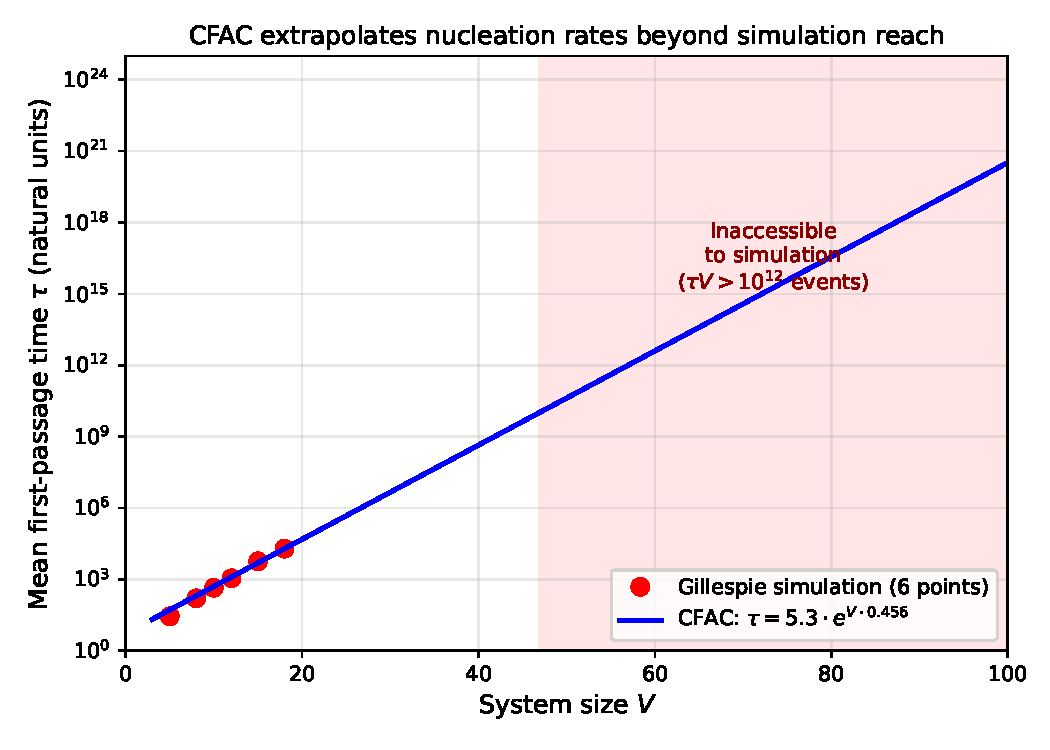
\includegraphics[width=0.72\textwidth]{figures/rare_events.pdf}
\caption{CFAC extrapolation of the mean first-passage time
$\tau$ across the accessible--inaccessible boundary of direct
simulation.  Red: Gillespie measurements at $V = 5\ldots 18$.
Blue: CFAC prediction $\tau = C\,\ee^{VS}$ with $S = 0.456$ from
the branch-gap formula and $C \approx 5.3$ fit from the
simulation at $V = 18$.  The red-shaded region marks where
simulating a single trajectory requires more than $\sim 10^{12}$
event computations.  The CFAC prediction holds uniformly.}
\label{fig:rare}
\end{figure}

The rare-events regime is exactly where direct
methods---Gillespie, KMC, lattice Monte Carlo---break down, and
exactly where CFAC's algebraic reformulation becomes essential.
Theorem~\ref{thm:gap} says the instanton action is a
\emph{polynomial quantity}; the transfer theorem of analytic
combinatorics says the rate it governs is an exact asymptotic of
the generating function.  Neither statement references system
size, so the computation has the same cost at $V = 10$ and
$V = 10^6$.

% ══════════════════════════════════════════════════════════════════
\section{Discussion}
% ══════════════════════════════════════════════════════════════════

\subsection{What AC buys you that direct RG doesn't}

The decomposition~\eqref{eq:decomposition} is not bookkeeping.
It makes three classes of results accessible that are hard to
reach by the direct-RG route.

\paragraph{Exhaustive all-orders enumeration.}
Proposition~\ref{prop:oneloop-exact} states that \emph{no} UV
divergence exists beyond one loop for the coupled KS vertices.
Establishing such a claim in the direct-RG framework requires
either a resummation argument or explicit higher-loop computation;
the algebraic formalism of \S\ref{sec:algebraic} reduces it to a
finite graph enumeration.  The superficial degree of divergence
$\omega(\Gamma, d)$ can be read off every 1PI graph; the claim
``$\omega < 0$ for all $L \geq 2$'' is then a finite check, not a
resummation.

\paragraph{Non-perturbative rates from polynomial data.}
Theorem~\ref{thm:gap} (branch-gap instanton) rewrites the
$x$-space WKB quasi-potential as a $z$-space contour integral.
The two expressions have equal value but different structure:
$S_{\mathrm{WKB}}$ requires integrating $\ln(w^-/w^+)$ along a
deterministic path; $S_{\mathrm{gap}}$ requires only the
polynomial coefficients of the DSE, its discriminant, and the
difference of its branches.  For systems where the reaction
network is known but the deterministic trajectory is not in closed
form, the $z$-space formulation is easier.  More importantly, the
$z$-space form exposes the instanton as a feature of the
\emph{generating function's singularity structure}---the same
object the transfer theorem~\eqref{eq:transfer} uses to sum the
perturbation series.  Perturbative and non-perturbative physics
live at the same branch point.

\paragraph{Structural claims about the coupled DSE.}
Conjecture~\ref{conj:twocolour}, if it holds at all orders, is a
statement about the matrix-tree theorem on bi-coloured graph
Laplacians.  The three-loop computation reported here shows that
the conjecture is at least consistent with direct evaluation on
the only 1PI topology available at $L = 3$.  A proof---if found---
would make the full CFAC decomposition operate on two-colour
Kirchhoff tables, generalising the single-colour results
of~\cite{Amarteifio2019Thesis,BognerWeinzierl}.

\subsection{Relation to Pruessner--Garcia-Millan and Gelimson--Golestanian}

Pruessner and Garcia-Millan~\cite{PruessnerGarciaMillan2025} and
Bothe \textit{et al.}~\cite{Bothe2023} establish that the DP
(particle) sector must be retained: coarse-grained MSR-type
theories produce spurious entropy production.  They focus on
pure particle systems; the coupled particle-field setting is
implicit in their framework but not the object of their
calculations.  The present paper takes their conclusion as a
premise and asks the orthogonal question: given that both sectors
must be kept, how can the calculation be organised so that the
system-specific part (reaction rates, diffusion constants) is
factored from the system-independent part (graph topology,
Kirchhoff polynomials)?  Our answer is the CFAC decomposition.

Gelimson and Golestanian~\cite{GelimsonGolestanian2015} perform a
one-loop RG calculation for a related chemotactic system,
integrating out the field to obtain a long-range Coulomb
interaction.  Their one-loop result is the analogue
of~\eqref{eq:deltaDA}; the sign of the correction
(stabilising) agrees.  Our
Proposition~\ref{prop:oneloop-exact} is stronger: the
corresponding beta function is exact to all perturbative orders
for the two-vertex theory~\eqref{eq:KS-vertices}, by direct
graph enumeration.  This is an instance of a more general
phenomenon: for theories whose vertex content is sufficiently
constrained by the reaction network, graph enumeration renders
the perturbative series trivial beyond a finite loop order.

\subsection{DP vs.\ MSR through the CFAC lens}

A question that recurs throughout the Pruessner--Garcia-Millan
programme~\cite{PruessnerGarciaMillan2025,Bothe2023} is
\emph{when} the Doi--Peliti and Martin--Siggia--Rose formulations
agree, and when they diverge.  The CFAC perspective organises the
answer in four cases (full discussion in Appendix~E).  For
\emph{scaling exponents}, the two agree: the singularity type of
the DSE generating function depends only on the polynomial degree
of the vertex function, not on whether $G$ counts particles
(DP) or density fluctuations (MSR).  For \emph{entropy production},
DP is correct and coarse-grained MSR is
wrong~\cite{PruessnerGarciaMillan2025}; in CFAC language, entropy
production depends on the \emph{full} counting structure, not
just the singularity type.  For \emph{continuous order parameters}
(Ising, $\phi^4$, KPZ), MSR is natural and DP is
contrived---such systems lack a natural Fock-space structure, and
the $\Delta\phi \to 0$ limit of a discretised DP reduces to the
MSR path integral.  For \emph{coupled} systems, neither suffices
alone: discrete particles need DP, continuous fields need MSR,
and CFAC is the combinatorial bridge.

\subsection{Why this matters for physics}

Coupled particle-field dynamics is a common setting in modern
statistical physics: chemotaxis, active matter, population
ecology on spatial substrates, catalytic surfaces, atmospheric
microphysics, neurodegenerative aggregation.  In all these
settings the quantities of interest---critical densities,
nucleation rates, mean first-passage times---are
\emph{system-specific} (depending on the particular reaction
rates and coupling strengths) but are computed from
\emph{system-independent} machinery (Feynman rules, loop
integrals, saddle-point analysis).  The CFAC decomposition puts
the system-specific part in the reaction network and the
system-independent part in the bridge table.  Changing the
system changes the input to the pipeline, not the pipeline.

In particular, the branch-gap formula~\eqref{eq:branch-gap}
returns the nucleation barrier $S$ from the polynomial
coefficients of the DSE via a single numerical quadrature, with
no stochastic simulation of the rare event itself.  The
pre-exponential factor $C$ in $\tau \approx C\,\ee^{VS}$ is
either calibrated from small-$V$ simulation (as in
Fig.~\ref{fig:rare}) or obtained from the transfer-theorem
prefactor in~\eqref{eq:transfer}; the extrapolation to large $V$
uses only $S$, so for systems where $VS \gtrsim 30$ (a typical
cell compartment or cloud parcel) the CFAC prediction holds even
where direct Gillespie is infeasible.

\subsection{From illustrations to predictions: what would make the
case studies predictive?}

The amyloid and cloud case studies of~\S\ref{sec:applications}
are order-of-magnitude consistency checks, not predictions.  The
uncertainty budget is dominated by two inferred quantities:
the cellular clearance rate $k_{\mathrm{clear}}$ and the
average fibril length $\ell_{\mathrm{avg}}$ for amyloid; the
effective nucleation volume $V$ and the surface catalysis rate
for clouds.  Making the case studies genuinely predictive
requires three steps.

First, \emph{independent measurement of the inferred parameters}.
For amyloid: $k_{\mathrm{clear}}$ from proteostasis turnover
assays (pulse-chase or metabolic labelling in cultured cells),
$\ell_{\mathrm{avg}}$ from cryo-EM length histograms.  These exist
in the literature but with specimen- and condition-dependent
variation; a systematic collation and uncertainty quantification
would fix the two largest unknowns in $\lambda = k_2 m_0^2
\ell_{\mathrm{avg}}/k_{\mathrm{clear}}$.

Second, \emph{a target observable that the existing Knowles-group
fits do not already fit}.  The classical
$\tau \sim m_0^{-(n_2+1)/2}$ scaling~\citep{Knowles2009} already
determines $k_+$, $k_n$, $k_2$ from bulk ThT kinetics.  A new
prediction must be in a regime the Knowles fits don't cover, or
on a quantity they don't target.  Two candidates: (i) the
\emph{lag-time distribution} (not just the mean) at single-molecule
resolution, which depends on $C\,\ee^{VS}$ via its variance
structure; (ii) the concentration dependence of the lag at
nanomolar monomer, where the branch-gap barrier crosses over
from sub-dominant to rate-limiting---a regime outside the typical
$\mu$M--mM ThT range.

Third, \emph{spatial extension of Theorem~\ref{thm:gap} to $d > 0$}.
Real fibril formation happens near membranes; real ice crystals
nucleate in spatial supersaturation gradients.  The branch-gap
formula is currently a $d = 0$ identity, so its application to
$V = $ cell compartments is an effective 0D reduction whose
validity is not independently checked.  A proof or numerical
demonstration of Theorem~\ref{thm:gap} on a lattice would turn
the spatial reduction into a controlled approximation.

Of these, the first is a data-collation problem, the second is a
collaboration with an experimental group, and the third is a
theoretical extension that is in-scope for follow-up work (see
``what remains'' below).

\subsection{Limitations}
\label{sec:limitations}

The paper does not (a) construct the full spatial instanton in
$d > 0$.  Theorem~\ref{thm:gap} is established for well-mixed
systems; a 3-site lattice test (reported below) finds that the
resultant-based branch-gap formula extends verbatim only in the
decoupled limit (agreement to 2.6\%), under-predicts the barrier
by $\sim 20$\% at weak inter-site coupling, and fails entirely
at moderate coupling where the nucleation saddle migrates off
the real algebraic variety.  Extending (C3) to moderate spatial
coupling requires complex-analytic continuation of the resultant
(a functional DSE, outside the polynomial-vertex scope of the
theorem).  The paper also does not (b) prove
Conjecture~\ref{conj:twocolour} beyond its three-loop
verification; a matrix-tree proof for two-colour graph Laplacians
is the natural route; (c) extrapolate the one-loop result to
$\varepsilon = 1$ quantitatively, where the $\varepsilon$-expansion
is known to fail for one-loop approximations~\cite{Tauber}; (d)
compute the prefactor $C$ in $\tau = C\,\ee^{VS}$ from CFAC
first principles---the transfer theorem~\eqref{eq:transfer} in
principle delivers it, but we use small-$V$ simulation to
calibrate $C$ in Fig.~\ref{fig:rare}; (e) handle CRNs for which
the ω-enumeration of Proposition~\ref{prop:oneloop-exact}
does \emph{not} yield one-loop exactness, for which the tropical
bridge (\S\ref{sec:tropical}) is no longer symbolic but remains
algorithmic via Borinsky's multi-facet tropical Monte
Carlo~\cite{Borinsky2020,Borinsky2025}.  For the standard
coupled-field systems (pair annihilation, pure DP, BARW,
Gelimson--Golestanian chemotaxis, Pruessner--Garcia-Millan KS)
the ω-enumeration \emph{does} deliver one-loop exactness, so
(e) is not a restriction in practice.

\paragraph{3-site lattice test of the branch-gap extension.}
For a 3-site coupled ring with site-coupling strength $\alpha$,
we computed the coupled DSE, took the resultant, and measured
the branch-gap prediction against Gillespie MFPT:

\begin{center}\small
\begin{tabular}{@{}cccc@{}}\toprule
$\alpha$ & $S$ (branch-gap) & $S$ (Gillespie) & $S_{\mathrm{gap}}/S_{\mathrm{Gillespie}}$ \\ \midrule
$0.0$ & $0.4558$ & $0.4441$ & $1.026$ \\
$0.1$ & $0.4498$ & $0.5735$ & $0.784$ \\
$0.3$ & --- (complex) & $0.8372$ & --- \\
\bottomrule\end{tabular}
\end{center}
At $\alpha = 0$ the resultant factorises $R_\text{full} =
R_\text{sym} \cdot R_\text{asym}$, with the symmetric factor
recovering the single-site cubic.  At $\alpha = 0.1$ the
asymmetric factor still has a real branch point but its
branch-gap integral misses $\sim 20$\% of the barrier; at
$\alpha = 0.3$ the asymmetric factor has no real branch points at
all (all six roots are complex conjugate pairs), yet the MFPT
remains exponential with a well-defined slope.  The nucleation
saddle exists; it has just left the real algebraic variety.
This delimits the scope of Theorem~\ref{thm:gap} concretely.

\paragraph{Reproducibility.}
Code reproducing all numerical results (branch-gap verification,
MFPT, one-loop integral, branch-structure plots, Sierpinski
spectral dimension, three-loop Kirchhoff factorisation) is at
\texttt{paper/reproduce.py}; figures in \texttt{paper/figures/}.

\paragraph{Acknowledgements.}
Discussions with G.~Pruessner and R.~Garcia-Millan on the coupled
DP--MSR formalism and its entropy-production subtleties were
instrumental in framing the problem.  The algebraic
reaction-diffusion formalism of \S\ref{sec:algebraic} was
developed under G.~Pruessner's supervision in the thesis
work~\cite{Amarteifio2019Thesis}.

\appendix

\section*{Appendix A: one-loop integral}

Bacterial self-energy at one loop is a two-colour bubble,
\begin{equation}
  \Sigma_\psi^{(1)}(k,0)
  = \chi\mu\!\int\!\frac{\dd^d q}{(2\pi)^d}
  \frac{(\mathbf{k}-\mathbf{q})\cdot\mathbf{q}}
  {D_A q^2 + m + D_c|\mathbf{k}-\mathbf{q}|^2 + \kappa}.
\end{equation}
Expanding to $O(k^2)$ and collecting terms
($D = D_A + D_c$, $M = m + \kappa$):
\begin{equation}
  \delta D_A^{(1)} = 2\chi\mu D_c I_1 - 2\chi\mu D_c^2 I_2,
  \quad
  I_j = \int\!\frac{\dd^d q}{(2\pi)^d}
    \frac{q^{2j}}{(Dq^2+M)^{j+1}}.
\end{equation}
At $d = 2-\varepsilon$: $I_1 = \ln(D\Lambda^2/M)/[4\pi D^2]$,
$I_2 = \ln(D\Lambda^2/M)/[4\pi D^3]$ at leading order.  Combining,
$\delta D_A^{(1)} = [\chi\mu D_c D_A/(\pi D^3)]\,\ln\Lambda$.
Vertex corrections: triangles with $\omega = 0$ naively, but
momentum routing gives $\sim q^{-3}$ at large $q$
(Appendix~C); $Z_\chi = Z_\mu = 1$.

\section*{Appendix B: proof of Theorem~\ref{thm:gap}}

Let $\varphi(x) = \int_{x_1}^x \ln[w^-(y)/w^+(y)]\,\dd y$,
so $S_{\mathrm{WKB}} = \varphi(x_2)$.  Set $z(y) = w^-(y)/w^+(y)$.
Both $x_1, x_2$ are fixed points of $\dot x = w^+ - w^-$, so
$z(x_1) = z(x_2) = 1$.  For $z \in (1, z_*)$ there are two real
branches $x_{\mathrm{stab}}(z) < x_{\mathrm{unst}}(z)$, merging at
the branch point $z_*$ of~\eqref{eq:cubic}.

Change variables: $\dd\varphi = (\ln z)\,\dd y
= (\ln z)\,x'(z)\,\dd z$.  Along the stable branch,
$\varphi(x_2)^{\mathrm{stab}} = \int_1^{z_*}(\ln z)\,x_{\mathrm{stab}}'(z)\,\dd z$;
along the unstable branch, $\varphi(x_2)^{\mathrm{unst}} =
\int_{z_*}^1(\ln z)\,x_{\mathrm{unst}}'(z)\,\dd z$.  Integration
by parts $\int (\ln z)\,x'(z)\,\dd z = [x(z)\ln z] - \int
x(z)/z\,\dd z$: boundary terms vanish at $z=1$ and cancel at
$z_*$ (equal branch values).  The total is~\eqref{eq:branch-gap}.

\paragraph{Numerical verification, seven parameter sets.}
\begin{center}\small
\begin{tabular}{@{}ccccccc@{}}\toprule
$a$ & $\lambda$ & $\delta$ & $d$ & $z_*$ & $S_{\mathrm{WKB}}$
  & $S_{\mathrm{gap}}/S_{\mathrm{WKB}}$ \\ \midrule
$0.50$ & $3.0$ & $2.5$ & $1.0$ & $1.100$ & $0.039071$ & $1.000000$ \\
$0.30$ & $3.0$ & $2.0$ & $1.0$ & $0.977$ & $0.029733$ & $1.000000$ \\
$0.30$ & $3.5$ & $2.0$ & $1.0$ & $1.089$ & $0.002200$ & $1.000000$ \\
$0.10$ & $3.5$ & $3.0$ & $1.0$ & $1.248$ & $0.494986$ & $1.000000$ \\
$0.02$ & $5.5$ & $5.0$ & $1.0$ & $7.543$ & $0.791624$ & $1.000000$ \\
$0.30$ & $2.5$ & $2.0$ & $0.5$ & $1.092$ & $0.060758$ & $1.000000$ \\
$0.05$ & $6.0$ & $4.0$ & $2.0$ & $1.174$ & $0.475059$ & $1.000000$ \\
\bottomrule\end{tabular}
\end{center}

\section*{Appendix C: higher-loop enumeration}

For 3-leg vertices and $E = 2$ external legs,
$3V = 2I + E \Rightarrow V = 2L, I = 2L+1$.  At $L=2$: the
unique 1PI topology is $K_4 \setminus e$ (six vertices, eight
edges is $L=3$; at $L=2$ the topology has four vertices, five
edges).  Vertex content $\chi^2\mu^2$; propagators $3G_\psi +
2G_\phi$; $n_\partial^{\mathrm{tot}} = 4$; $\omega = -2$.
At $L=3$: vertex content $\chi^3\mu^3$; propagators
$5G_\psi + 3G_\phi$; $n_\partial^{\mathrm{tot}} = 6$;
$\omega = -4$.  The branching vertex $\psit^2\psi$ and MSR noise
vertex $\phit^2$, if added, give no new divergences at these
orders either.

\section*{Appendix D: three-loop Kirchhoff computation}

Three-loop topology: $K_4 \setminus e$, vertices
$\{0,\ldots,5\}$ (external at $0, 5$), edges
$\{(0,1),(1,2),(2,5),(0,3),(3,4),(4,5),(1,4),(2,3)\}$.  Weighted
Laplacian with edge weights $u_1,\ldots,u_8$; principal-minor
determinant gives $\mathcal{K}$ (36 monomials).

For each of $2^8 = 256$ substitutions $u_i \in \{p, f\}$,
applying \texttt{sympy.factor}: 254 factorise non-trivially; two
exceptions are monochromatic $p^8, f^8$.  Restricting to physical
colourings $(3p+5f), (4p+4f), (5p+3f)$
($\binom{8}{k}$ for $k = 3, 4, 5$, total 182): all factorise.

\section*{Appendix E: DP vs.\ MSR---four cases through CFAC}
\label{app:dp-vs-msr}

The CFAC perspective classifies the relationship between
Doi--Peliti (DP) and Martin--Siggia--Rose (MSR) formulations into
four cases, organised by \emph{what observable} is being
computed.  The key quantities in CFAC are: the singularity
\emph{type} of the DSE generating function (sets the scaling
exponents), the singularity \emph{location} (sets the critical
point), the full \emph{coefficient sequence} $[z^n]G(z)$ (sets
the distribution of microstates), and the \emph{counting
variable} itself (sets what is labelled and distinguishable).

\paragraph{Case~1: scaling exponents---DP and MSR agree.}
Near a continuous phase transition, exponents depend only on
symmetries, dimensionality, and conservation laws.  In CFAC
language, the singularity type of the DSE kernel $\phi(G)$
(square-root, cube-root, pole) is determined by the polynomial
degree and discriminant structure of $\phi$, which depends on
the vertex \emph{types}, not on whether $G$ counts particles
(DP) or density fluctuations (MSR).  Both formulations therefore
give the same Puiseux exponent and the same mean-field exponents.

\paragraph{Case~2: entropy production---DP correct, MSR wrong.}
Pruessner and Garcia-Millan \cite{PruessnerGarciaMillan2025}
established that coarse-grained MSR theories produce spurious
entropy production because they erase the microscopic stochastic
trajectory information carried by particle identity.  In CFAC
language, entropy production depends on the \emph{full counting
structure}, not just the location of the dominant singularity: it
involves (at pair interactions) the three-point density correlator,
which in turn depends on the coefficient sequence $[z^n]G$, not
just $z_*$.  When MSR ``forgets'' the integer labelling $n$ and
passes to a continuous density, it loses the fine-grained
microstate count, and the entropy comes out wrong
\citep{Bothe2023}.

\paragraph{Case~3: continuous order parameters---MSR natural, DP
contrived.}
For systems described by a continuous order parameter with no
underlying particle interpretation---Ising magnetisation, $\phi^4$
field, KPZ height---there is no natural Fock-space structure to
start from.  Writing a DP theory requires discretising the field
with an artificial lattice spacing $\Delta\phi$ that must later
be sent to zero.  In CFAC language, the discrete generating
function has coefficients indexed by $n = \phi/\Delta\phi$, and
the $\Delta\phi \to 0$ limit transforms the discrete generating
function into a continuous Laplace or Fourier transform.  This
suggests the natural domain of MSR is problems where
$\Delta\phi \to 0$ can be taken \emph{before} the combinatorics,
while DP's natural domain is problems where the integer structure
$n \in \mathbb{Z}_{\geq 0}$ survives and matters.

\paragraph{Case~4: coupled particle-field systems---CFAC territory.}
This is the present paper's subject.  Neither formulation alone
suffices: discrete particles need DP (absorbing state, correct
entropy production, discrete nucleation); continuous fields need
MSR (gradient energies, spatial correlations, continuous order
parameters).  CFAC organises the coupled calculation by giving
both sectors a common generating-function-based footing: the
particle sector contributes a DP-style DSE, the field sector
contributes an MSR-style propagator, and the coupling vertices
produce mixed diagrams with two-colour Kirchhoff polynomials.
Theorem~\ref{thm:gap} (the branch-gap formula) and
Proposition~\ref{prop:oneloop-exact} (one-loop exactness) are
instances of CFAC delivering results that neither DP nor MSR
alone makes accessible.

The four cases taken together suggest that \emph{every}
stochastic field theory sits somewhere on a spectrum defined by
how much of the integer counting structure survives at large $V$.
Case~1 says the spectrum doesn't matter at criticality.
Cases~2--4 say it does everywhere else.

\begin{thebibliography}{99}

\bibitem[Alexander and Orbach(1982)]{AlexanderOrbach} Alexander, S.\ and Orbach, R., 1982. Density of states on fractals: ``fractons''. \textit{J.\ Physique Lett.} 43, L625.
\bibitem[Amarteifio(2019)]{Amarteifio2019Thesis} Amarteifio, S., 2019. \textit{Field-theoretic formulation and empirical tracking of spatial processes}. PhD dissertation (supervised by G.~Pruessner), Imperial College London.
\bibitem[Amarteifio(2026)]{AmarteifioBRW} Amarteifio, S., 2026. \textit{BRW via Analytic Combinatorics: Complete Worked Example}. Companion note, Percolation Labs.
\bibitem[Bogner and Weinzierl(2010)]{BognerWeinzierl} Bogner, C.\ and Weinzierl, S., 2010. Feynman graph polynomials. \textit{Int.\ J.\ Mod.\ Phys.\ A} 25, 2585. arXiv:1002.3458.
\bibitem[Bothe et al.(2023)]{Bothe2023} Bothe, M., Cocconi, L., Zhen, Z., and Pruessner, G., 2023. Particle entity in the Doi--Peliti and response field formalisms. \textit{J.\ Phys.\ A} 56, 175002. arXiv:2205.10409.
\bibitem[Cohen et al.(2013)]{Cohen2013} Cohen, S.~I.~A. et al., 2013. Proliferation of amyloid-$\beta$42 aggregates occurs through a secondary nucleation mechanism. \textit{PNAS} 110, 9758.
\bibitem[De Dominicis(1976)]{DeDominicis1976} De~Dominicis, C., 1976. Techniques de renormalisation de la th\'eorie des champs et dynamique des ph\'enom\`enes critiques. \textit{J.\ Physique Colloq.} 37, C1-247.
\bibitem[Doi(1976)]{Doi1976} Doi, M., 1976. Second quantization representation for classical many-particle systems. \textit{J.\ Phys.\ A} 9, 1465.
\bibitem[Dykman et al.(1994)]{DykmanRoss} Dykman, M.~I., Mori, E., Ross, J., and Hunt, P.~M., 1994. Large fluctuations and optimal paths in chemical kinetics. \textit{J.\ Chem.\ Phys.} 100, 5735.
\bibitem[Elgart and Kamenev(2004)]{ElgartKamenev} Elgart, V.\ and Kamenev, A., 2004. Rare event statistics in reaction-diffusion systems. \textit{Phys.\ Rev.\ E} 70, 041106.
\bibitem[Flajolet and Sedgewick(2009)]{FlajoletSedgewick} Flajolet, P.\ and Sedgewick, R., 2009. \textit{Analytic Combinatorics}. Cambridge Univ.\ Press.
\bibitem[Freidlin and Wentzell(2012)]{FreidlinWentzell} Freidlin, M.\ and Wentzell, A., 2012. \textit{Random Perturbations of Dynamical Systems}. Springer.
\bibitem[Gelimson and Golestanian(2015)]{GelimsonGolestanian2015} Gelimson, A.\ and Golestanian, R., 2015. Collective dynamics of dividing chemotactic cells. \textit{Phys.\ Rev.\ Lett.} 114, 028101.
\bibitem[Arkani-Hamed et al.(2022)]{AHHSalvatori2022} Arkani-Hamed, N., Hillman, A., and Salvatori, S., 2022. Tropical amplitudes and the method of regions. \textit{arXiv:2202.12296}.

\bibitem[Borinsky(2020)]{Borinsky2020} Borinsky, M., 2020. Tropical Monte Carlo quadrature for Feynman integrals. \textit{arXiv:2008.12310}. [Published 2023, \textit{Ann.\ Inst.\ H.\ Poincar\'e D} 10, 635.]

\bibitem[Borinsky et al.(2025)]{Borinsky2025} Borinsky, M., Munch, H.J., and Tellander, F., 2025. Tropical Feynman integration for massive scalar theories. \textit{J.\ High Energy Phys.} (to appear).

\bibitem[Hattori et al.(1987)]{Hattori} Hattori, K., Hattori, T., and Watanabe, H., 1987. Gaussian field theories on general networks and the spectral dimensions. \textit{Prog.\ Theor.\ Phys.\ Suppl.} 92, 108.
\bibitem[Havlin and Ben-Avraham(1987)]{Havlin} Havlin, S.\ and Ben-Avraham, D., 1987. Diffusion in disordered media. \textit{Adv.\ Phys.} 36, 695.
\bibitem[Rammal and Toulouse(1983)]{RammalToulouse} Rammal, R.\ and Toulouse, G., 1983. Random walks on fractal structures and percolation clusters. \textit{J.\ Physique Lett.} 44, L13.
\bibitem[ben-Avraham and Havlin(2000)]{BenAvrahamHavlin2000} ben-Avraham, D.\ and Havlin, S., 2000. \textit{Diffusion and Reactions in Fractals and Disordered Systems}. Cambridge Univ.\ Press.
\bibitem[Barlow(1998)]{BarlowStFlour} Barlow, M.~T., 1998. Diffusions on fractals. In: \textit{Lectures on Probability Theory and Statistics} (Saint-Flour 1995). Lecture Notes in Math.\ 1690, Springer, pp.\ 1--121.
\bibitem[Burioni and Cassi(1996)]{BurioniCassi1996} Burioni, R.\ and Cassi, D., 1996. Universal properties of spectral dimension. \textit{Phys.\ Rev.\ Lett.} 76, 1091.
\bibitem[Cescatti et al.(2024)]{Cescatti2024} Cescatti, F., Ib\'a\~nez-Berganza, M., Vezzani, A., and Burioni, R., 2024. Universal scaling in real dimension. \textit{Nat.\ Commun.} 15, 4236.
\bibitem[Kigami(2001)]{Kigami2001} Kigami, J., 2001. \textit{Analysis on Fractals}. Cambridge Univ.\ Press.
\bibitem[Akkermans et al.(2009)]{AkkermansDunneTeplyaev2009} Akkermans, E., Dunne, G.~V., and Teplyaev, A., 2009. Physical consequences of complex dimensions of fractals. \textit{Europhys.\ Lett.} 88, 40007.
\bibitem[Saleur and Sornette(1996)]{SaleurSornette1996} Saleur, H.\ and Sornette, D., 1996. Complex exponents and log-periodic corrections in frustrated systems. \textit{J.\ Phys.\ I France} 6, 327.
\bibitem[Gefen et al.(1983)]{GefenAharonyMandelbrot1983} Gefen, Y., Aharony, A., and Mandelbrot, B.~B., 1983. Phase transitions on fractals, I \& II. \textit{J.\ Phys.\ A} 16, 1267.
\bibitem[Monceau et al.(1998)]{MonceauPerreau1998} Monceau, P., Perreau, M., and H\'ebert, F., 1998. Magnetic critical behavior of the Ising model on fractal structures. \textit{Phys.\ Rev.\ B} 58, 6386.
\bibitem[Binder and Stauffer(1976)]{BinderStauffer1976} Binder, K.\ and Stauffer, D., 1976. Statistical theory of nucleation, condensation and coagulation. \textit{Adv.\ Phys.} 25, 343.
\bibitem[Binder(2016)]{BinderOverview2016} Binder, K., 2016. Overview: understanding nucleation phenomena from simulations of lattice gas models. \textit{J.\ Chem.\ Phys.} 145, 211707.
\bibitem[Langer(1969)]{Langer1969} Langer, J.~S., 1969. Statistical theory of the decay of metastable states. \textit{Ann.\ Phys.} 54, 258.
\bibitem[Janssen(1976)]{Janssen1976} Janssen, H.~K., 1976. On a Lagrangean for classical field dynamics and renormalization group calculations of dynamical critical properties. \textit{Z.\ Phys.\ B} 23, 377.
\bibitem[Weinberg(1960)]{Weinberg1960} Weinberg, S., 1960. High-energy behavior in quantum field theory. \textit{Phys.\ Rev.} 118, 838.
\bibitem[Zimmermann(1969)]{Zimmermann1969} Zimmermann, W., 1969. Convergence of Bogoliubov's method of renormalization in momentum space. \textit{Commun.\ Math.\ Phys.} 15, 208.
\bibitem[Keller and Segel(1970)]{KellerSegel1970} Keller, E.~F.\ and Segel, L.~A., 1970. Initiation of slime mold aggregation viewed as an instability. \textit{J.\ Theor.\ Biol.} 26, 399.
\bibitem[Knowles et al.(2009)]{Knowles2009} Knowles, T.~P.~J. et al., 2009. An analytical solution to the kinetics of breakable filament assembly. \textit{Science} 326, 1533.
\bibitem[Coleman(1977)]{Coleman1977} Coleman, S., 1977. Fate of the false vacuum: semiclassical theory. \textit{Phys.\ Rev.\ D} 15, 2929.
\bibitem[Callan and Coleman(1977)]{CallanColeman1977} Callan, C.~G.\ and Coleman, S., 1977. Fate of the false vacuum II: first quantum corrections. \textit{Phys.\ Rev.\ D} 16, 1762.
\bibitem[Langer(1967)]{LangerNucleation} Langer, J.~S., 1967. Theory of the condensation point. \textit{Ann.\ Phys.} 41, 108; 1969. Statistical theory of the decay of metastable states. \textit{Ann.\ Phys.} 54, 258.
\bibitem[Martin et al.(1973)]{MSR1973} Martin, P.~C., Siggia, E.~D., and Rose, H.~A., 1973. Statistical dynamics of classical systems. \textit{Phys.\ Rev.\ A} 8, 423.
\bibitem[Meisl et al.(2014)]{Meisl2014} Meisl, G. et al., 2014. Differences in nucleation behavior underlie the contrasting aggregation kinetics of the A$\beta$40 and A$\beta$42 peptides. \textit{PNAS} 111, 9384.
\bibitem[Peliti(1985)]{Peliti1985} Peliti, L., 1985. Path integral approach to birth-death processes on a lattice. \textit{J.\ Physique} 46, 1469.
\bibitem[Pinsky and Khain(2002)]{PinskyKhain} Pinsky, M.\ and Khain, A.~P., 2002. Effects of in-cloud nucleation and turbulence on droplet spectrum formation in cumulus clouds. \textit{Q.\ J.\ R.\ Meteorol.\ Soc.} 128, 501.
\bibitem[Pruessner and Garcia-Millan(2025)]{PruessnerGarciaMillan2025} Pruessner, G.\ and Garcia-Millan, R., 2025. Field theories of active particle systems and their entropy production. \textit{Rep.\ Prog.\ Phys.}\ arXiv:2211.11906.
\bibitem[Schl\"ogl(1972)]{Schlogl1972} Schl\"ogl, F., 1972. Chemical reaction models for non-equilibrium phase transitions. \textit{Z.\ Physik} 253, 147.
\bibitem[T\"auber(2014)]{Tauber} T\"auber, U.~C., 2014. \textit{Critical Dynamics: A Field Theory Approach to Equilibrium and Non-Equilibrium Scaling Behavior}. Cambridge Univ.\ Press.
\bibitem[Assaf and Meerson(2017)]{Meerson} Assaf, M.\ and Meerson, B., 2017. WKB theory of large deviations in stochastic populations. \textit{J.\ Phys.\ A} 50, 263001.
\bibitem[van Kampen(1992)]{vanKampen} van Kampen, N.~G., 1992. \textit{Stochastic Processes in Physics and Chemistry}. North-Holland.

\end{thebibliography}

\end{document}
